\pdfoutput=1

%-------------------------------------------------------------------------------%
%                         DOCUMENT CLASS AND PACKAGES                           %
%-------------------------------------------------------------------------------%

% Document class
\documentclass[aps,twocolumn,amsmath,amssymb,preprintnumbers,floatfix,prl,superscriptaddress,longbibliography]{revtex4-2}%{revtex4}%

% Font and encoding
\usepackage[utf8]{inputenc}
\usepackage{newtxtext}
\usepackage[upint]{newtxmath}
\usepackage{microtype}
\usepackage{textcomp}
\usepackage{eucal}
\usepackage{bm}
\usepackage{siunitx}
\usepackage{comment}
\usepackage{lipsum}


% Notation
\usepackage{enumerate}
\usepackage{amsfonts}
\usepackage{amsmath}
\usepackage{amssymb}
\usepackage{color}
\usepackage{soul}

% Figures
\usepackage{graphicx}

% References
\usepackage[colorlinks,allcolors=blue]{hyperref}
\usepackage[capitalize]{cleveref}
\newcommand{\crefrangeconjunction}{--}



%-------------------------------------------------------------------------------%
%                                CUSTOM MACROS                                  %
%-------------------------------------------------------------------------------%

% Ensure consistent notation

\definecolor{DarkRed}{rgb}{0.65,0,0}%
\definecolor{Green}{rgb}{0,0.3,0.3}
\definecolor{Purple}{rgb}{0.3,0,0.65}
\definecolor{Red}{rgb}{1,0,0}
\definecolor{Blue}{rgb}{0,0,0.85}
\definecolor{Magenta}{rgb}{1,0,1}



%% Math
\newcommand{\Imag}{{\Im\mathrm{m}}}   % Imaginary part 
\newcommand{\Real}{{\mathrm{Re}}}   % Real part
\newcommand{\im}{\mathrm{i}}        % Imaginary unit non-italic
\newcommand{\ve}[1]{\boldsymbol{#1}}
\DeclareMathOperator{\diag}{diag} % Requires amsopn.sty (included in amsmath)
\newcommand{\x}{\lambda}  % holder for plus/minus 1 (\pm 1)
\newcommand{\y}{\rho}     % holder for plus/minus 1 (\pm 1)
\newcommand{\T}{\mathrm{T}}   % Time ordering operator
\newcommand{\Pv}{\mathcal{P}} % Principal value operator
\newcommand{\mf}{m_\text{F}} 
\newcommand{\ms}{m_\text{S}} 
\newcommand{\vk}{{\ve{k}}} % Vector k
\newcommand{\vecA}{\ve{A}} % Vector k
\newcommand{\hvec}{\ve{h}} % Vector k
\newcommand{\vech}{\ve{h}} % Vector k
\newcommand{\vecf}{\ve{f}} % Vector k



\newcommand{\ow}{odd-$\omega$ } % Vector k
\newcommand{\ew}{even-$\omega$ } % Vector k

\newcommand{\hatx}{\hat{\boldsymbol{x}}} % Vector k
\newcommand{\haty}{\hat{\boldsymbol{y}}} % Vector k
\newcommand{\hatz}{\hat{\boldsymbol{z}}} % Vector k

%\newcommand{\ot}{~\overset{\circ}{ , }~}

\newcommand{\vs}{\vec{\sigma}} % Vector p\newcommand{\vp}{\ve{p}} % Vector p\

\newcommand{\vpf}{\mathbf{\vp}_\text{F}} % Vector pF
\newcommand{\xx}{\mathcal{X}} 
\newcommand{\vq}{\ve{q}} % Vector q
\newcommand{\vg}{\ve{g}} % Vector q
\newcommand{\ca}[2][]{c_{#2}^{\vphantom{\dagger}#1}} % op. c (annihilate) 
\newcommand{\cc}[2][]{c_{#2}^{{\dagger}#1}}          % op. c dagger (create) 
\newcommand{\da}[2][]{d_{#2}^{\vphantom{\dagger}#1}} % op. d (annihilate) 
\newcommand{\dc}[2][]{d_{#2}^{{\dagger}#1}}          % op. d dagger (create) 
\newcommand{\ga}[2][]{\gamma_{#2}^{\vphantom{\dagger}#1}} % op. gamma
\newcommand{\ea}[2][]{\eta_{#2}^{\vphantom{\dagger}#1}} % op. eta
\newcommand{\ec}[2][]{\eta_{#2}^{{\dagger}#1}}          % op. eta dagger 

\newcommand{\dn}{\downarrow}
\newcommand{\up}{\uparrow}
\newcommand{\ph}{\phantom{\dag}}

\newcommand{\Tkp}[1]{T_{\vk\vp#1}}  % Tunneling matrix element
\newcommand{\muone}{\mu^{(1)}}      % Chem.pot. side one
\newcommand{\mutwo}{\mu^{(2)}}      % Chem.pot. side two
\newcommand{\epsk}{\varepsilon_\vk}
\newcommand{\epsp}{\varepsilon_\vp}
\newcommand{\e}[1]{\mathrm{e}^{#1}}
\newcommand{\dif}{\mathrm{d}} %Rett d i differensial
\newcommand{\diff}[2]{\frac{\dif#1}{\dif#2}}%Derivert
\newcommand{\mean}[1]{\langle#1\rangle}
\newcommand{\abs}[1]{|#1|}
\newcommand{\abss}[1]{|#1|^2}
\newcommand{\Sk}[1][\vk]{\ve{S}_{#1}}
\newcommand{\pauli}[1][\alpha\beta]{\boldsymbol{\sigma}_{#1}^{\vphantom{\dagger}}}
\newcommand{\paulivec}{\mathbf{\hat{\sigma}}}
\newcommand{\nabtil}{\tilde{\nabla}}
\newcommand{\xh}{\ve{\hat{x}}}
\newcommand{\yh}{\ve{\hat{y}}}
\newcommand{\zh}{\ve{\hat{z}}}
\newcommand{\vecsigma}{\boldsymbol{\sigma}}

\newcommand{\veci}{{\ve{i}}}
\newcommand{\vecj}{{\ve{j}}}
\newcommand{\veck}{\ve{k}}
\newcommand{\vecn}{\ve{n}}
\newcommand{\vecd}{\ve{d}}
\newcommand{\vecx}{\ve{x}}
\newcommand{\vecy}{\ve{y}}

\newcommand{\vecr}{\ve{r}}
\newcommand{\vecp}{\ve{p}}
\newcommand{\vecq}{{\ve{q}}}
\newcommand{\vece}{\ve{e}}
\newcommand{\vecg}{\ve{g}}
\newcommand{\vecm}{\ve{m}}

\newcommand{\vecH}{\ve{H}}
\newcommand{\vecB}{\ve{B}}
\newcommand{\vecM}{\ve{M}}
\newcommand{\vecS}{\ve{S}}

\newcommand{\fd}{f(E_{nk}/2)}

\newcommand{\gc}{\check{g}}

%% Text
\newcommand{\eq}{Eq.}%No extra space when used with reftex (->auto ~)
\newcommand{\eqs}{Eqs.}%No extra space when used with reftex (->auto ~)
\newcommand{\cf}{\textit{cf. }}%adv : that is to say; in other words
\newcommand{\ie}{\textit{i.e. }}%adv : that is to say; in other words
\newcommand{\eg}{\textit{e.g. }}%[syn: f.eks., for example, for instance]
\newcommand{\etal}{\emph{et al.}}
\def\i{\mathrm{i}}                            

\newcommand{\ppartial}{\bar{\partial}}

\newcommand{\g}{\underline{\gamma}}
\newcommand{\gt}{\underline{\tilde{\gamma}}}
\newcommand{\N}{\underline{\mathcal{N}}}
\newcommand{\Nt}{\underline{\tilde{\mathcal{N}}}}

\newcommand{\be}{\begin{equation}}
\newcommand{\ee}{\end{equation}}

\newcommand*{\ou}[2]{\overset{\text{\large ${#1}$}}{#2}}

\newcommand\comdot{%
  \mathrel{{\ooalign{\hss\raisebox{-0.3ex}{$,$}\hss\cr\raisebox{0.3ex}{$\cdot$}}}}
}

\newcommand\combullet{%
  \mathrel{{\ooalign{\hss\raisebox{-0.3ex}{$,$}\hss\cr\raisebox{0.3ex}{$\bullet$}}}}
}

\newcommand\comtimes{%
  \mathrel{{\ooalign{\hss\raisebox{-0.3ex}{$,$}\hss\cr\raisebox{0.3ex}{$\times$}}}}
}

\newcommand{\vehsigma}{\hat{\ve{\sigma}}}
\newcommand{\vesigma}{\ve{\sigma}}
\newcommand{\vep}{\ve{p}}
\newcommand{\veq}{\ve{q}}
\newcommand{\vgf}{\ve{q}_{F}}
\newcommand{\hrhot}{\hat{\rho}_{3}}
\newcommand{\hrhoz}{\hat{\rho}_{0}}
\newcommand{\veR}{\ve{R}}
\newcommand{\ver}{\ve{r}}
\newcommand{\hnabla}{\hat{\nabla}}


% Other macros
\newcommand{\prlsection}[1]{\textit{#1}.\kern0.05em---\kern0.05em\ignorespaces}

% For collaborative editing
\newcommand{\hans}[1]{\textcolor{Magenta}{{#1}}}
\newcommand{\jacob}[1]{\textcolor{Red}{{#1}}}


% 
\usepackage{subcaption} % to use subfigures
% \usepackage{todonotes} % to add to do-notes
\usepackage{comment}
% \usepackage{biblatex}
% \addbibresource{bibliography.bib}

%-------------------------------------------------------------------------------%
%                          TITLE PAGE AND ABSTRACT                            %
%-------------------------------------------------------------------------------%

\begin{document}
\title{Superconductor-altermagnet memory device without stray fields}
\author{Hans Gløckner Giil}
\affiliation{Center for Quantum Spintronics, Department of Physics, Norwegian \\ University of Science and Technology, NO-7491 Trondheim, Norway}

\author{Jacob Linder}
\affiliation{Center for Quantum Spintronics, Department of Physics, Norwegian \\ University of Science and Technology, NO-7491 Trondheim, Norway}


\begin{abstract}
\lipsum[1][1-20]



\end{abstract}
\maketitle

\textit{Introduction}---
The interplay of superconductivity and magnetism is a  major research topic in modern condensed matter physics. Its allure stems both from a fundamental viewpoint and cryogenic technology applications such as extremely sensitive detectors of radiation and heat as well as circuit components such as qubits and dissipationless diodes.  

Whereas superconductor/ferromagnet structures have been studied extensively, antiferromagnetic materials have received less attention. A particularly interesting example is recently discovered antiferromagnets that break time-reversal symmetry and feature a spin-splitting that does not originate from relativistic effects such as spin-orbit coupling. Dubbed altermagnets in the literature, these are spin-compensated magnetic systems with a huge momentum-dependent spin splitting even in collinearly ordered antiferromagnets. \textit{Ab initio} calculations have identified several possible material candidates that can host an altermagnetic state, including metals like RuO$_2$ and Mn$_5$Si$_3$ as well as semiconductors/insulators like MnF$_2$ and La$_2$CuO$_4$ 
\cite{yuan_prb_20, lopez-moreno_pccp_16, smejkal_sciadv_20, reichlova_arxiv_20, smejkal_prx_22}.

Superconducting memory devices with infinite magnetoresistance have been proposed and observed \cite{li_prl_13} using superconducting spin-valves. This is a trilayer structure consisting of one superconductor and two ferromagnets. The critical temperature $T_c$ of the superconductor is controlled by the relative magnetization orientation. In this way, $T_c$ changes up to 1 K have been reported \cite{singh_prx_15}.

The property enabling the functionality of such structure via external fields is also its drawback, depending on the precise mode of operation: the magnetization. The disadvantage is the inevitable existence of a stray field surrounding the structure, which limits how closely multiple structures of this type can be packed together without disturbing each other. Therefore, finding a way to control $T_c$ in a structure without any net magnetization could offer a major advantage to the implementation of such architecture in cryogenic devices.
The question arises how the recently proposed spin-split antiferromagnets affect the critical temperature of nearby superconductors, and whether they can have potential applications in such devices. 
Recent advances in the understanding of the altermagnet/superconductivity interplay \cite{sun_arx_23, ouassou_arx_23} have shown that such systems hold promise in controlling the supercurrent passing through the superconducting material. 

In this paper, we investigate the effect of the altermagnetic spin splitting on a nearby superconductor. We explore different geometries and device layouts, and the role of impurities in the antiferromagnetic material. 



\begin{comment}
\textit{Introduction}. The interaction between magnetism and superconductivity is a major research topic in modern condensed matter physics. Its allure stems both from a fundamental viewpoint and cryogenic technology applications such as extremely sensitive detectors of radiation and heat as well as circuit components such as qubits and dissipationless diodes. 

Whereas superconductor/ferromagnet structures have been studied extensively, antiferromagnetic materials have received less attention. A particularly interesting example is recently discovered antiferromagnets that break time-reversal symmetry and feature a spin-splitting that does not originate from relativistic effects such as spin-orbit coupling. Dubbed altermagnets in the literature, these are spin-compensated magnetic systems with a huge momentum-dependent spin splitting even in collinearly ordered antiferromagnets. \textit{Ab initio} calculations have identified several possible material candidates that can host an altermagnetic state, including metals like RuO$_2$ and Mn$_5$Si$_3$ as well as semiconductors/insulators like MnF$_2$ and La$_2$CuO$_4$ 
\cite{yuan_prb_20, lopez-moreno_pccp_16, smejkal_sciadv_20, reichlova_arxiv_20, smejkal_prx_22}.

There exists an interesting analogy between altermagnets and unconventional superconductivity in the high-$T_c$ cuprates where the order parameter has a $d$-wave symmetry in momentum space. Similarly, the band structure of altermagnets has a spin-resolved $d$-wave symmetry which mimicks the structure of the $d$-wave superconducting order parameter (see Fig. \ref{fig:model}). 

Superconducting memory devices with infinite magnetoresistance have been proposed and observed \cite{li_prl_13} using superconducting spin-valves. This is a trilayer structure consisting of one superconductor and two ferromagnets. The critical temperature $T_c$ of the superconductor is controlled by the relative magnetization orientation. In this way, $T_c$ changes up to 1 K have been reported \cite{singh_prx_15}.

The property enabling the functionality of such structure via external fields is also its drawback, depending on the precise mode of operation: the magnetization. The disadvantage is the inevitable existence of a stray field surrounding the structure, which limits how closely multiple structures of this type can be packed together without disturbing each other. Therefore, finding a way to control $T_c$ in a structure without any net magnetization could offer a major advantage to implementation of such architecture in cryogenic devices.
\end{comment}

\textit{Theory}---
The lattice Bogoliubov--de\,Gennes (BdG) method \cite{zhu2016, degennes1966} is suitable to study altermagnet/superconductor heterostructures, where the complicated form of the altermagnetic Hamiltonian makes e.g. a treatment using the Usadel equation difficult. 
We employ a mean-field Hamiltonian including altermagnetism and impurities,
\begin{equation}
\label{eq:Hn}
    \begin{split}
        H =&  E_0
		- \sum_{i\sigma} (\mu_i - w_i) c^\dag_{i\sigma} c_{i\sigma}
  - \sum_i (\Delta_i^{\vphantom{*}} c^\dag_{i\downarrow} c^\dag_{i\uparrow} 
    + \Delta_i^* c_{i\uparrow} c_{i\downarrow}) 
    \\& 
		- \sum_{\langle i, j \rangle \sigma} t_{ij} c^\dag_{i\sigma} c_{j\sigma}
		- \sum_{\langle i, j \rangle \sigma\sigma'} (\bm{m}_{ij} \cdot \bm{\sigma})_{\sigma\sigma'} c^\dag_{i\sigma} c_{j\sigma'}
    \end{split}
\end{equation}
where $c_{i\sigma}$ and $c^\dag_{i\sigma}$  destroy and create an electron with spin $\sigma$, $\mu_i$ is the chemical potential, $\Delta_i$ the (site-dependent) superconducting order parameter, $\bm{\sigma} = (\sigma_1, \sigma_2, \sigma_3)$ is the Pauli vector, and $w_i$ is an impurity potential, which we take to be randomly distributed at a given number of sites in the magnet.
For comparison, we consider two different forms of $\vec m_{ij}$: i) an on-site potential $\vec m_{ij} = m_z \delta_{ij} \hat z $, corresponding to a ferromagnetic term, and ii) $\bm{m}_{ij} = +m\bm{e}_z$ for nearest-neighbor hopping along the $x$ axis and $\bm{m}_{ij} = -m\bm{e}_z$ for hopping along the $y$ axis, corresponding to an effective altermagnetic term, similar to what was used in Ref. \onlinecite{ouassou_arx_23}. There is no antiferromagnetic order in the Hamiltonian \eqref{eq:Hn}, owing to the fact that this is an effective model, where antiferromagnetic order is removed by averaging over the unit cell.
We assume nearest neighbor hopping, i.e. $t_{ij} = t$, and scale all other parameters in units of $t$.
The order parameter can be determined from the site-dependent self-consistent gap equation,
\begin{equation}
    \label{eq:gapeeq}
    \Delta_i = U_i \langle c_{i \uparrow} c_{i \downarrow} \rangle
\end{equation}
Throughout the text, we set $\mu = -t/2$ and the attractive potential $U_i = 1.7t$.
The magnetic ters, order parameters, and impurity potential are only nonzero in their respective regions.

\textit{Methodology}---
\hans{Write about BDG-vectors u, v, about the solution strategy (binomial search, check if Delta increases etc).}

\begin{comment}
\textit{Theory}---
To model the proposed physical setup we employ the Bogoliubov--de\,Gennes (BdG) method \cite{zhu2016, degennes1966}.
Our starting point is a mean-field tight-binding Hamiltonian that includes altermagnetism and conventional superconductivity:
\begin{equation}\label{eq:H}
	\begin{aligned}
		H
		 & = E_0
		- \sum_{i\sigma} \mu_i c^\dag_{i\sigma} c_{i\sigma}
		- \sum_i (\Delta_i^{\vphantom{*}} c^\dag_{i\downarrow} c^\dag_{i\uparrow} 
    + \Delta_i^* c_{i\uparrow} c_{i\downarrow}) 
    \\
		 & \phantom{==}
		- \sum_{\langle i, j \rangle \sigma} t_{ij} c^\dag_{i\sigma} c_{j\sigma}
		- \sum_{\langle i, j \rangle \sigma\sigma'} (\bm{m}_{ij} \cdot \bm{\sigma})_{\sigma\sigma'} c^\dag_{i\sigma} c_{j\sigma'},
	\end{aligned}
\end{equation}
where $c_{i\sigma}$ and $c^\dag_{i\sigma}$ are the usual electronic annihilation and creation operators, and $\bm{\sigma} = (\sigma_1, \sigma_2, \sigma_3)$ is the Pauli vector.
$E_0$ describes a constant contribution which is not important for the self-consistent calculations below.
We choose constant nearest-neighbor hopping amplitudes~$t_{ij} \equiv t$ and chemical potentials~$\mu_i = -t/2$.
% In the two superconductors, we set $\Delta_i = \Delta e^{\pm i \delta\!\varphi/2}$.
% The gap was calculated using the interpolation formula $\Delta(T) \approx \Delta(0) \tanh\big[1.74 \sqrt{T_c/T - 1}\big]$,
% where we chose a zero-temperature gap $\Delta(0) = t/10$.
% The critical temperature was determined using the BCS ratio $\Delta(0)/T_c \approx 1.764$. 
The superconducting and altermagnetic terms in Eq. (\ref{eq:H}) are only present in their respective regions and are zero otherwise.
In the altermagnet, we set $\bm{m}_{ij} = +m\bm{e}_z$ for nearest-neighbor hopping along the $x$ axis and $\bm{m}_{ij} = -m\bm{e}_z$ for hopping along the $y$ axis.

This corresponds to a low-energy effective Hamiltonian $mk_xk_y\sigma_z$ or $m(k_x^2-k_y^2)\sigma_z$ \cite{yuan_prb_20, smejkal_prx_22}, depending on the crystallographic orientation of the sample.
This Hamiltonian differs from both the momentum-independent spin-splitting $m\sigma_z$ of a ferromagnet and a Rashba-type spin-orbit coupling
$mk_{x(y)}\sigma_z$.
\end{comment}


The fermionic operators at each site~$i$ can be grouped into Nambu vectors 
$\hat{c}_i \equiv (c_{i \up}^{\ph}, 
c_{i\dn}^{\ph}, c_{i\up}^\dag, c_{i\dn}^\dag)$
, which may in turn be collected into a $4N$-element vector $\check{c} \equiv (\hat{c}_1, \ldots, \hat{c}_N)$ containing every fermionic operator on the lattice.
The Hamiltonian operator can then be expressed via a $4N\times4N$ Hamiltonian matrix: $H = E_0 + \frac{1}{2} \check{c}^\dag \check{H} \check{c}$.
We solve the BdG equation by numerically diagonalizing $\check H$ and expressing physical observables such as the superconducting gap in \eq \eqref{eq:gapeeq} in terms of its eigenvectors and eigenvalues. 
This can be done by starting with a guess $\Delta_g$ for the gap parameter, and then self-consistently solving diagonalizing the Hamiltonian until the superconducting order parameter converges. However, here we are mainly interested in calculating the critical temperature $T_c$, and do not need the explicit numerical value of the gap. 
Thus, we do not explicitly calculate the order parameter but instead perform $N_\Delta$ self-consistent iterations, and compare the result with some small value $\Delta_g = 10^{-5}$. We define the material as superconducting when the median value inside the superconductor has increased compared with the initial value $\Delta_g$.
The critical temperature is then determined by performing a binomial search in temperatures, which is much faster than a linear search.

\begin{figure}[t!]
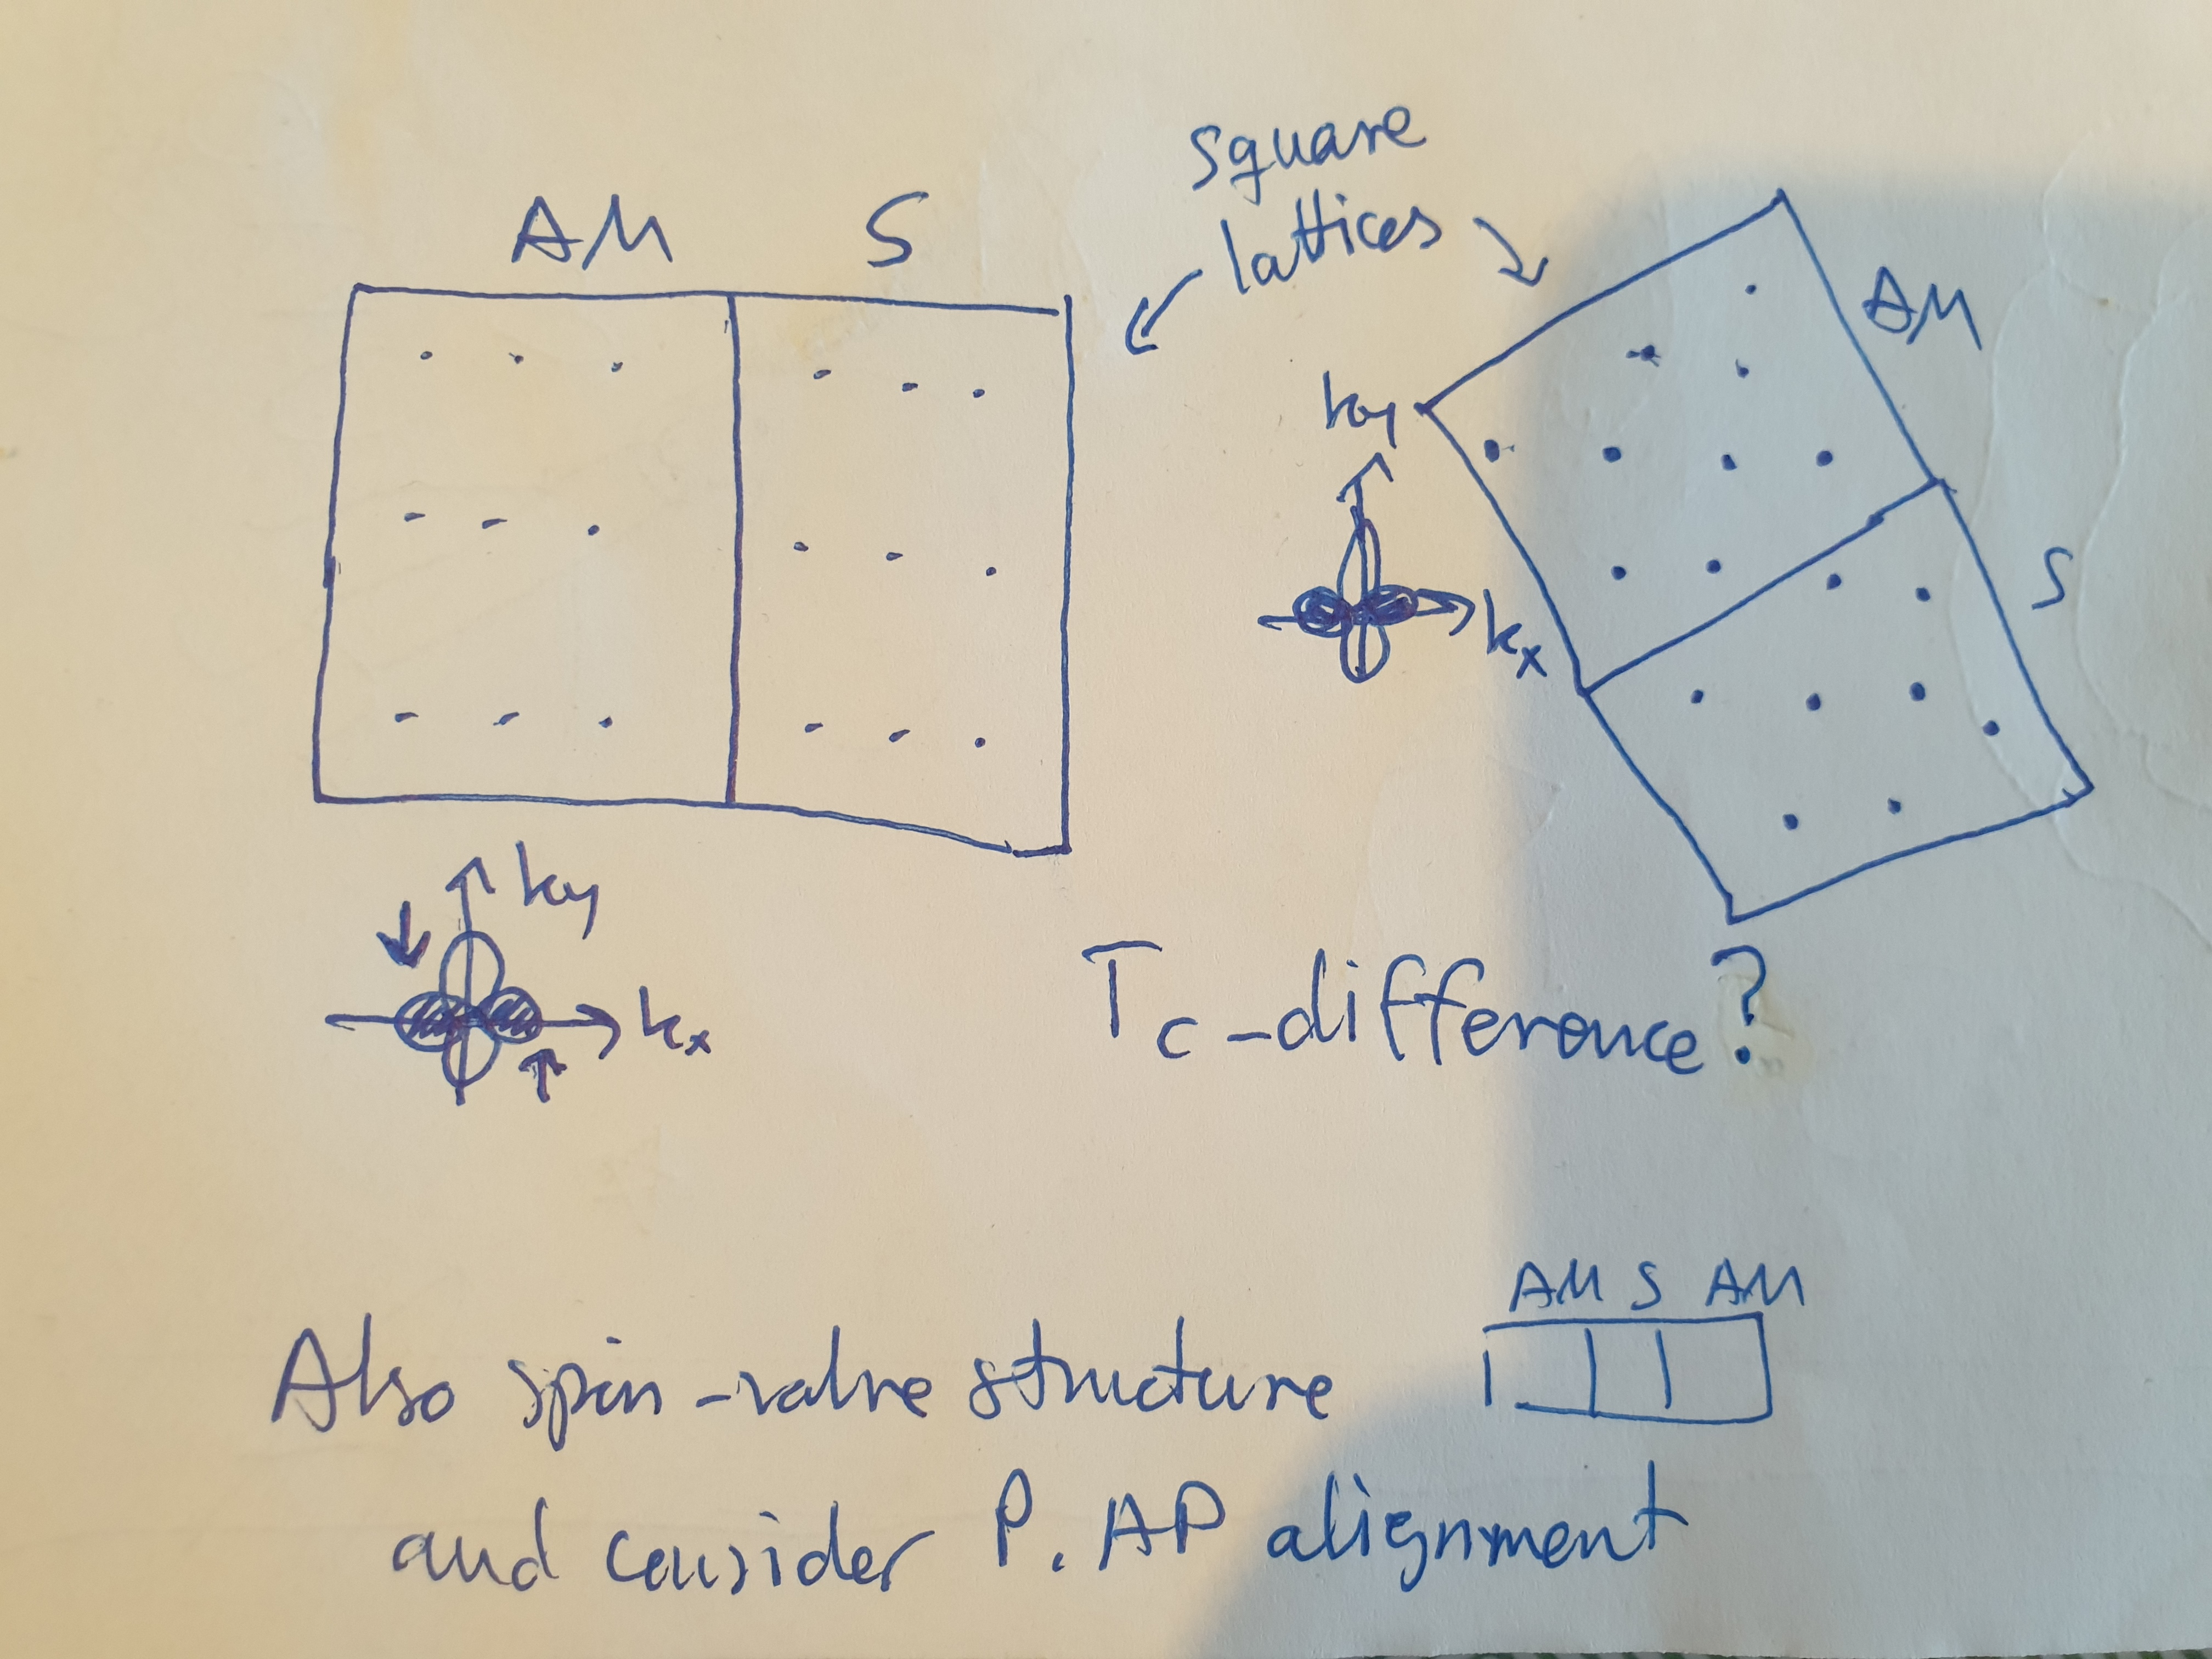
\includegraphics[width=0.87\columnwidth]{test.jpg}
	\caption{...
	}
	\label{fig:model}
\end{figure}
\text{ }\\
\text{ }\\


\noindent \textbf{Strategy and relevant references}\\
The idea is to compute how $T_c$ of a superconductor is changed when placed in proximity to an altermagnet. $T_c$ could change as a function of
\begin{itemize}
    \item The crystallographic orientation of the altermagnet relative the superconductor (straight vs diagonal junction in Fig. 1)
    \item The impurity concentration in the system. Impurities are added via an extra onsite term in $H$ with a random amplitude.
    \item The relative orientation (P and AP) of altermagnets in an AM/S/AM structure. 
    \item The superconducting order parameter symmetry ($s$-wave vs $d$-wave, as relevant for elemental superconductors like Nb or Al vs high-$T_c$ ones like YBCO, PCCO)
\end{itemize}
Moreover, we are able to include the role of interfacial spin-orbit coupling due to the Rashba effect by adding a corresponding term to $H$, if we like. This could also have an impact. 
\text{ }\\

See bdgnotes.pdf in this overleaf-folder for a nice introduction to diagonalization of the BdG equations on a lattice. 
\text{ }\\

I have access to supercomputer resources to speed up calculations if we need. 
\text{ }\\

\textit{Destruction of the superconducting order.}---
\begin{comment}
    \hans{COMMENT: I am not sure it is obvious why the altermagnetic strength is ''more effective'' in lowering $T_c$ than the exchange field.} \jacob{[COMMENT: I agree: in fact, the altermagnet term should like a $\vk$-dependent exchange field (see the other comment). If we thus compare $m[\cos(k_x) - \cos(k_y)]$ with $m$, the $k$-dependence should make the average value (averaged over Fermi surface) of the altermagnet term smaller than $m$. Wouldn't it make more sense that the altermagnet actually supports larger values of $m$ where SC can coexist with it than in the FM case where the spin-splitting is $m$ for all $\vk$-values? ]}
    \hans{Comment: This seems somewhat reasonable, but is this not assuming that the Fermi surface is (approximately ) the same after adding altermagnetism? In reality, it is changed (so that it is not invariant under $90 ^\circ$ rotations), see plot in Fig. \ref{fig:FS} below. But the altermagnetic strength $m = 0.04$ is not enough to drastically change the Fermi surface....
    Moreover, we have a factor 2 as well. } \jacob{[COMMENT: you're right, I assumed circular symmetry, which is not the case generally. That makes the effect on AM on the SC gap equation less straight-forward to infer, but, for the same reason, more interesting to clarify.]}
\end{comment}

% \begin{figure}
%     \centering
%     \begin{subfigure}{0.45\textwidth}
%         \includegraphics[]{}
%     \end{subfigure}
%     \caption{Caption}
%     \label{fig:enter-label}
% \end{figure}
Before studying heterostructures of superconductors and altermagnets, it is instructive first to understand the effects of the altermagnetic term in \eq \eqref{eq:Hn} on the superconducting order.
To this end, we consider a system with altermagnetic and superconducting order. We vary the altermagnetic strength $m$ and calculate the critical temperature self-consistently. The results are shown in Fig. \ref{fig:coex} and show that the effect of altermagnetism is to suppress the superconducting order, which vanishes for altermagnetic strength of $m \approx 0.3 \Delta_0$, where $\Delta_0$ is the zero-temperature and zero-field gap. The results are compared with the effects of ferromagnetism, which also suppresses the superconductivity in a similar way, although the critical field $h$ is much larger than in the altermagnetic case.
% \begin{figure}[htb]
%     \centering
%     \begin{subfigure}{0.7 \linewidth}
%         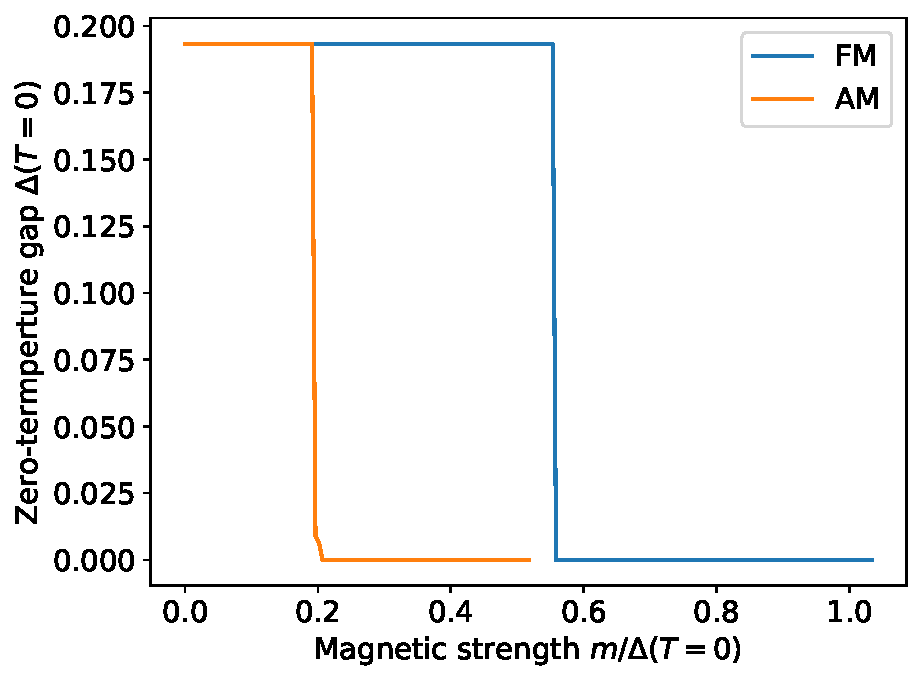
\includegraphics[width = \linewidth] {plots_maintext/onemat_Deltas.pdf}
%     \end{subfigure}
%     \begin{subfigure}{0.7 \linewidth}
%         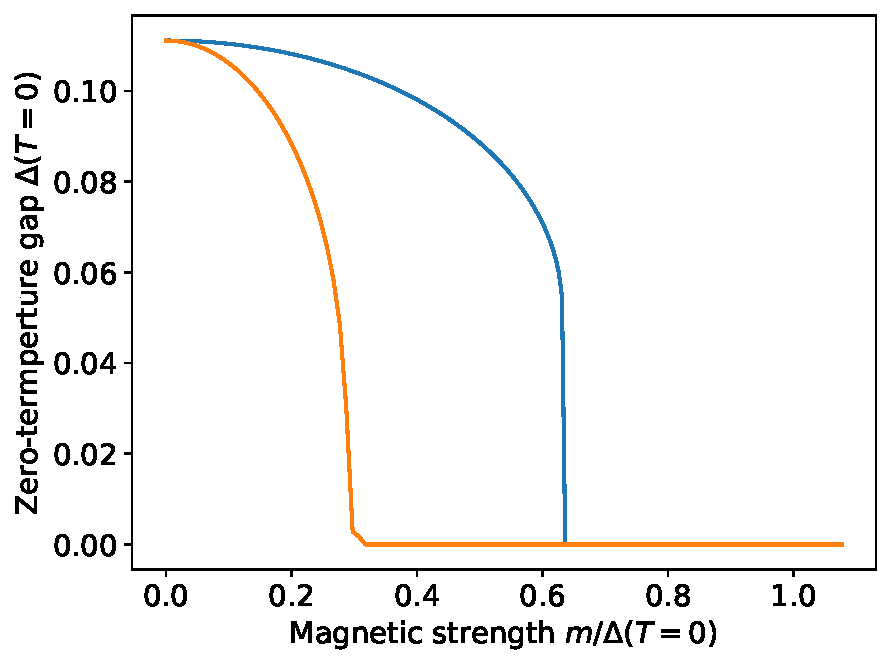
\includegraphics[width = \linewidth] {plots_maintext/onemat_Tcs.pdf}
%     \end{subfigure}
%     \caption{The effect of the altermagnetic term on superconductivity in a structure with coexisting magnetism and superconductivity, compared with the effect of ferromagnetism. In the left panel, the zero-temperature gap $\Delta(T = 0)$. In the right panel: the critical temperature as a function of the alter- and ferromagnetic strength.
%     Parameters used in both subplots are: $\mu = -0.5t$, $U = 1.7t$, $N_x = 20$, $N_y = 10$. The zero-field gap is $\Delta(T=0, m = 0) = 0.1934$, and the critical temperature is $T_c(m = 0) = 0.1096$.}
%     %\hans{\cite{chandrasekhar_apl_62, clogston_prl_62}. COMMENT: I will run this with much higher accuracy (to get smoother curves) in the end, if we decide to keep this plot.} \hans{To Do: add also several runs, for different chemical potentials $\mu$, see if they shift.} \hans{Todo 2: Compare with Chandrasekhar-Clogston limit. Also, can we do some analytical work here? \jacob{[COMMENT: yes, I think semi-analytical work can be done here. See section II in \url{https://arxiv.org/pdf/0707.4413.pdf} up to eq 11. Here, the gap equation for a spin-split superconductor is derived. The final step from eq 10 to eq 10 is obtained by differentiating the free energy with respect to $\Delta$, if I recall correctly (assuming $\Delta$ is real, otherwise one has to differentiate wrt $\Delta^*$. In our case, we consider coexistence of altermagnetism + SC. The first step is then to look at what the altermagnetic hopping term looks like in $\vk$-space by Fourier-transforming our real-space model. I think we should get something like $m\sin(k_x)\sin(k_y)$. Then, we just replace $h$ in eq. 2 in the above paper with $m[\cos(k_x) - \cos(k_y)]$. The rest of the derivation should be identical, we can get a gap equation of similar form as eq 11. This can then maybe be solved analytically in some limiting cases, and at least very quickly numerically. An advantage with this derivation is that we also have access to the free energy (eq 10) immediately: this is needed to check if the superconducting solution we find is in fact the ground-state. In other words, even if we find a self-consistent $\Delta \neq 0$, this is only the actual ground-state if the free energy for this solution is lower than the non-superconducting state. ]} \hans{I agree with your comment. I do think, however, that we cannot approximate the sum we find from differentiating eq (10) with an integral since the sum is not invariant under $k_x \leftrightarrow k_y$. We might need to perform the sum numerically.} \jacob{[COMMENT: yes, although we can still express the final gap equation as an integral over $k_X$ or $k_y$ instead of a sum, if that for some reason is beneficial.]}\hans{Yes, that is true.} \hans{It looks like the results are OK by just summing over $~1000$ values of $k_x$ and 1000 values of $k_y$ over the entire Brillouin zone, so maybe we don't have to do integral approximation. }
%     \label{fig:coex}
% \end{figure}
\begin{figure}[htb]
    \centering
    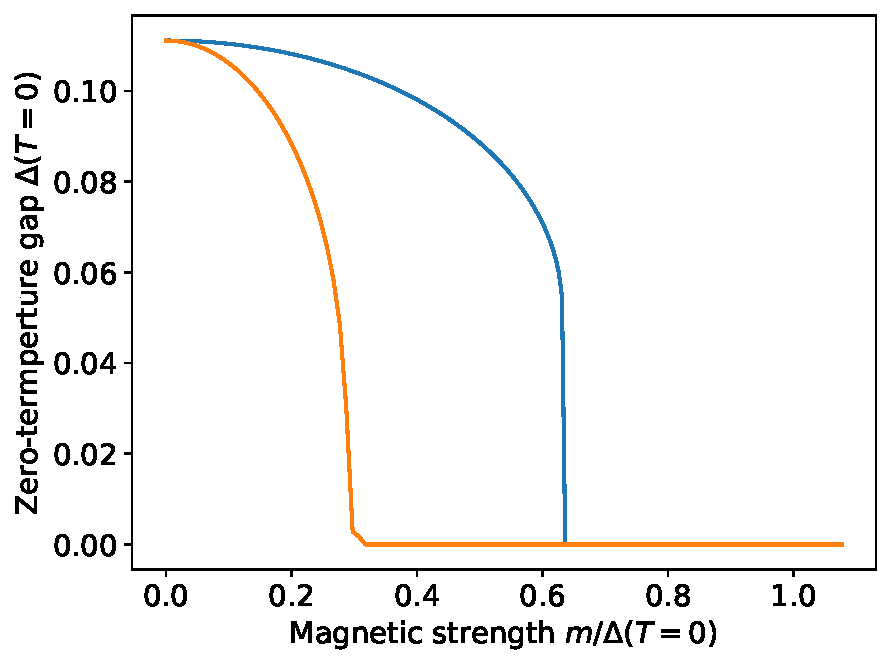
\includegraphics[width = 0.6\linewidth]{plots_maintext/onemat_Tcs.pdf}
    \caption{
    The critical temperature for a $N_x = 20$, $N_y = 20$ material as a function of the alter- and ferromagnetic strength in a structure of coexisting superconductivity and altermagnetic/ferromagnetic spin splitting.
    The zero-field and zero-temperature gap is $\Delta(T=0, m = 0) = 0.1949$.}
    \label{fig:coex}
\end{figure}
This is supported by a semi-analytical calculation, where we analytically found the gap equation for such a system, 
\begin{equation}
    g(\Delta) \equiv 1 - \frac{U}{2 N} \sum_{k_x, k_y} \frac{1 - f(E_{k_x k_y \uparrow}) - f(E_{k_x k_y \downarrow})}{\sqrt{\xi_\mathbf{k}^2 + \Delta^2}} = 0,
\end{equation}
where $N$ is the number of lattice sites in the system, and the (spin-dependent) eigenvalues are
\begin{equation}
    E_{k_x k_y \sigma} = \sqrt{\xi_{\mathbf{k}}^2 + \Delta^2}
    -\sigma( h  + 2m (\cos{k_x} - \cos{k_y})),
\end{equation}
and $\sigma = \pm $ is the spin. 
\hans{COMMENT: Can put the derivation for this in supplementary material if we decide to keep it in.}
We consider only the case of either ferromagnetism or altermagnetism, i.e. either $h= 0, m\neq 0$ or $h\neq 0, m= 0$. The gap equation is plotted for different values of $\Delta$ in the ferro- and altermagnetic case in Fig. \ref{fig:g}, together with the free energy density of the system. The plots show the same behavior for $\Delta$ as Fig. \ref{fig:coex} showed for $T_c$: the altermagnetic term $m$ suppresses the superconductivity, and the critical value is smaller than in the ferromagnet.
\hans{COMMENT: Perhaps better if I can find the critical temperature from the gap equation instead since we don't really talk about $\Delta_0$ anywhere else.}
\begin{figure}[htb]
    \centering
    \begin{subfigure}{0.49 \linewidth}
    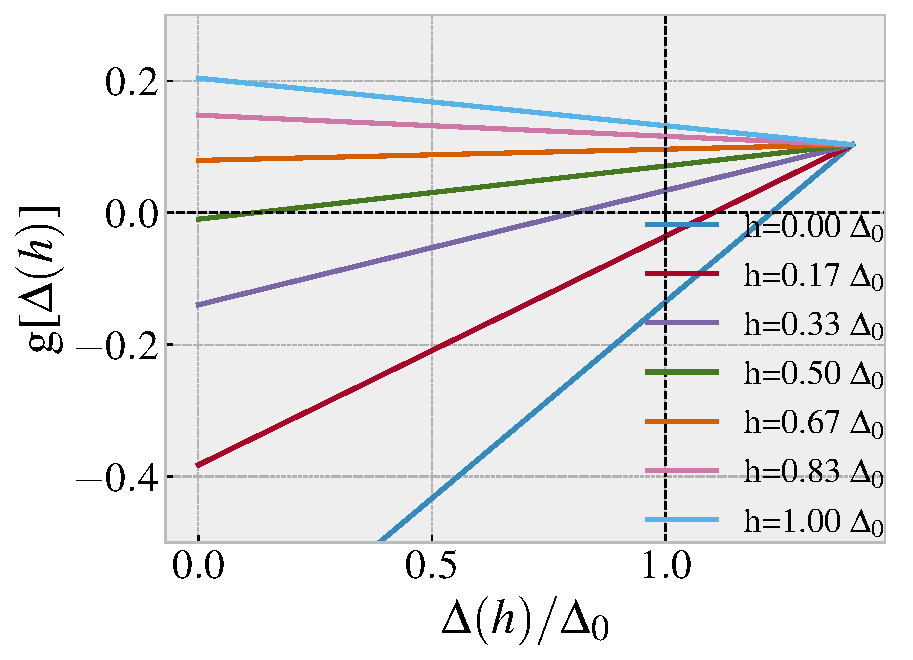
\includegraphics[width = \linewidth]{plots_maintext/g_hx_mu=-0.5_m=0.00_neghT=0.01.pdf}
    \end{subfigure}
    \begin{subfigure}{0.49 \linewidth}
    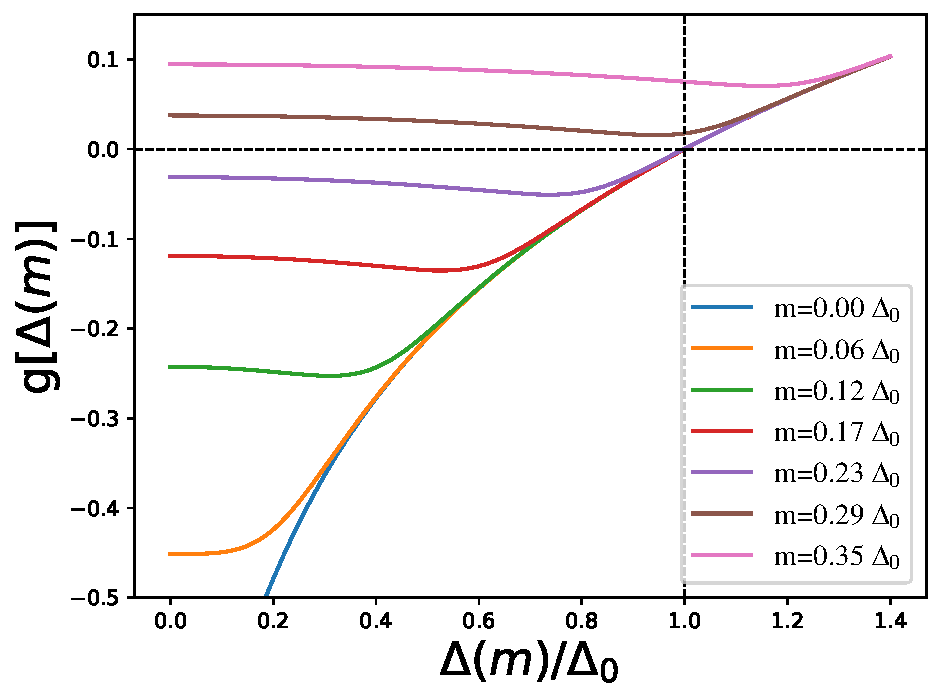
\includegraphics[width = \linewidth]{plots_maintext/g_m_mu=-0.5_h=0.00T=0.01.pdf}
    \end{subfigure}
    \begin{subfigure}{0.49 \linewidth}
            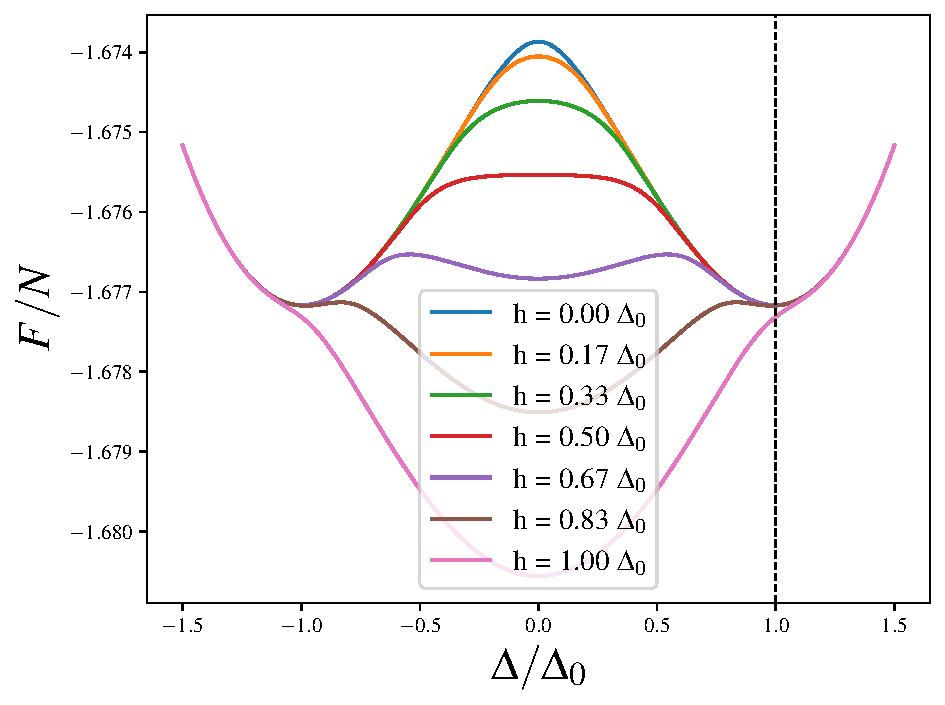
\includegraphics[width = \linewidth]{plots_maintext/F_hT=0.01.pdf}
    \end{subfigure}
    \begin{subfigure}{0.49 \linewidth}
        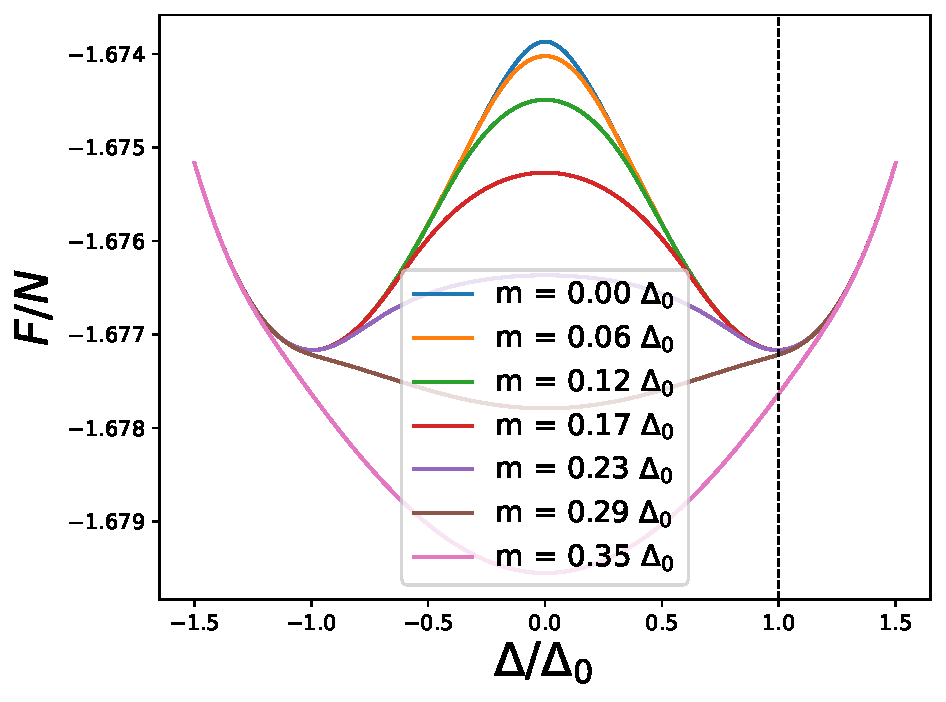
\includegraphics[width = \linewidth]{plots_maintext/F_mT=0.01.pdf}
    \end{subfigure}
    \caption{The solutions for the zero-temperature gap equation for different ferromagnetic and altermagnetic strength values. The solutions of the gap equation are given by the intersection of the curves with the (dashed) $x$-axis.
    The FM case is shown in the left panels, and the AM case is shown in the right panels. 
    % The solutions for the FM case are consistent with the results of \url{https://arxiv.org/pdf/0707.4413.pdf}.
    % The plots show that superconductivity is suppressed for smaller $m$ in an AM, compared to $h$ in a FM.
    The temperature was set to $T=0.05\Delta_0$, and the zero-temperature and zero-field gap was found to be $\Delta_0 = 0.1943$.}
    % ( the small deviation from the numerical BdG-results are thought to be because of the small system size in the numerical BdG case).}
    \label{fig:g}
\end{figure}
% \begin{figure}[htb]
%     \centering
%     \begin{subfigure}{0.49 \linewidth}
%     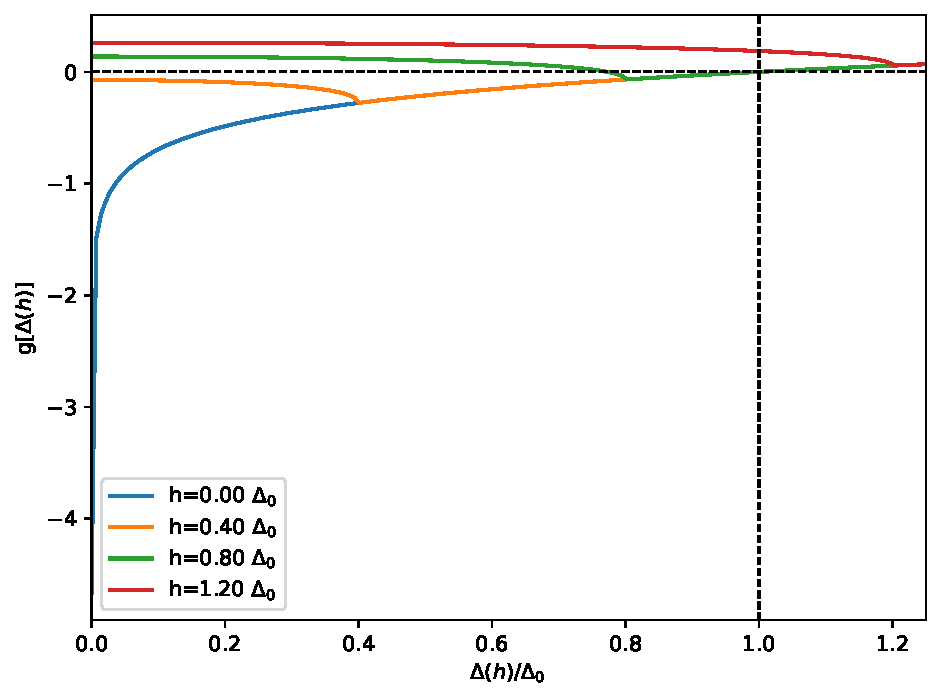
\includegraphics[width = \linewidth]{plots_maintext/g_h_mu=-0.5.pdf}
%     \end{subfigure}
%     \begin{subfigure}{0.49 \linewidth}
%     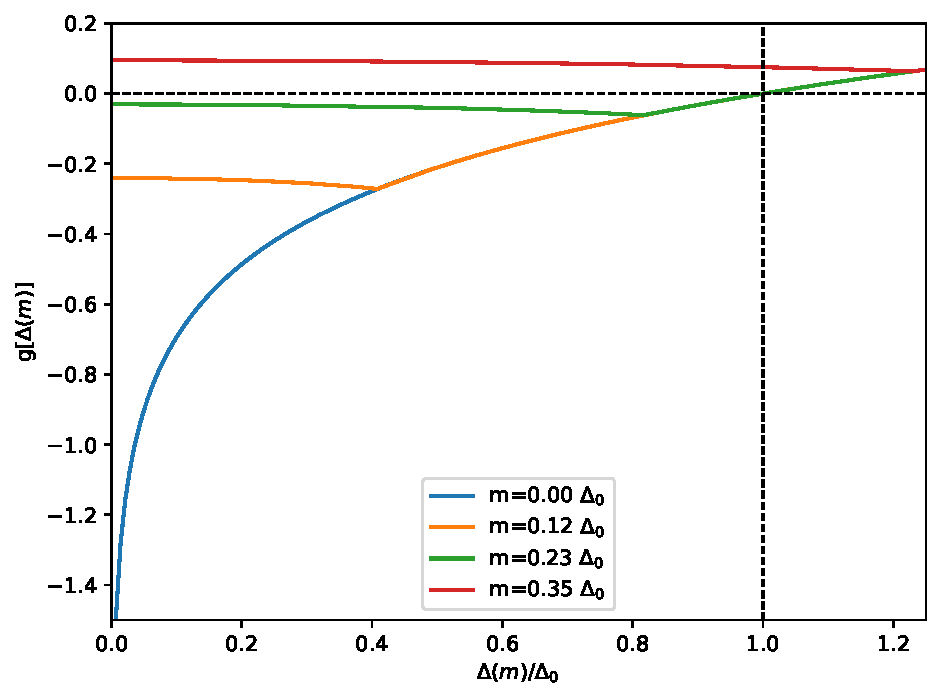
\includegraphics[width = \linewidth]{plots_maintext/g_m_mu=-0.5.pdf}
%     \end{subfigure}
%     \begin{subfigure}{0.49 \linewidth}
%             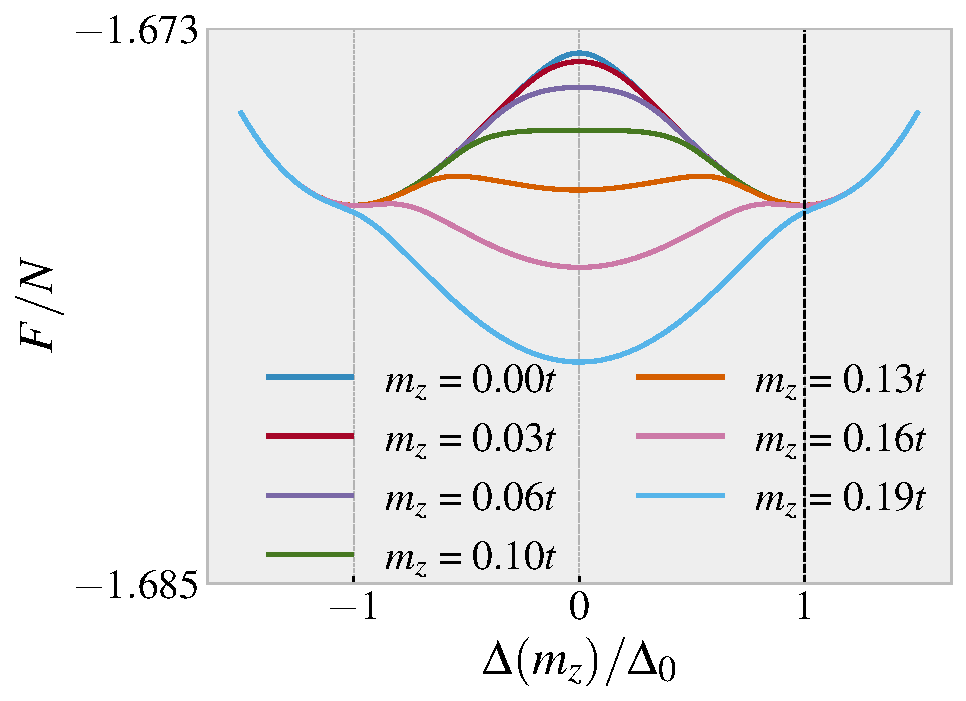
\includegraphics[width = \linewidth]{plots_maintext/F_h.pdf}
%     \end{subfigure}
%     \begin{subfigure}{0.49 \linewidth}
%         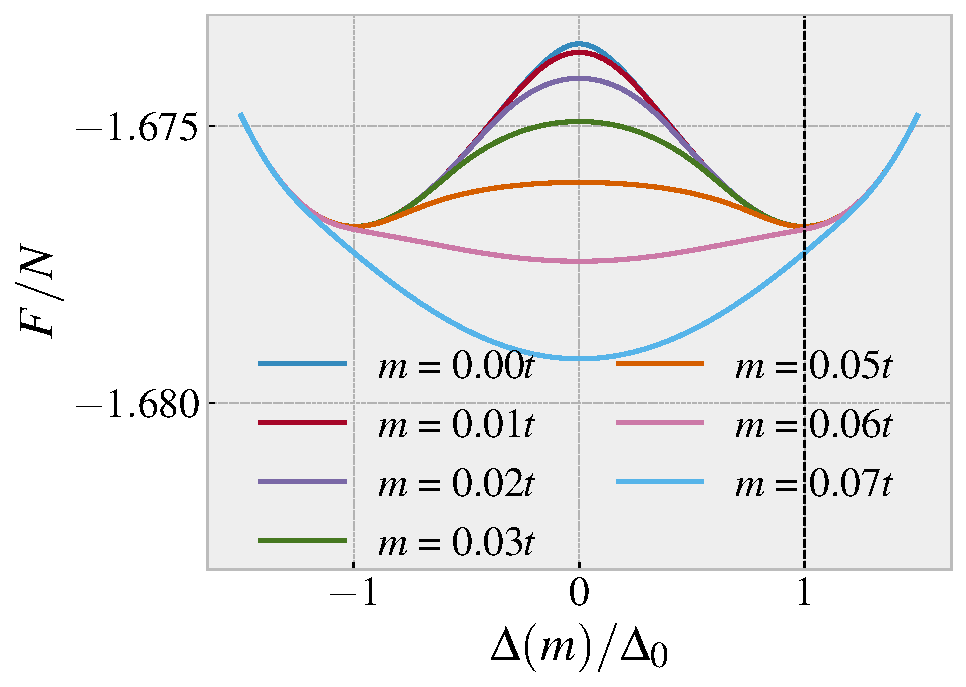
\includegraphics[width = \linewidth]{plots_maintext/F_m.pdf}
%     \end{subfigure}
%     \caption{The solutions for the zero-temperature gap equation for different ferromagnetic and altermagnetic strength values. The solutions of the gap equation are given by the intersection of the curves with the $y=0$-line.
%     The FM case is shown in the left panels, and the AM case is shown in the right panels. 
%     % The solutions for the FM case are consistent with the results of \url{https://arxiv.org/pdf/0707.4413.pdf}.
%     % The plots show that superconductivity is suppressed for smaller $m$ in an AM, compared to $h$ in a FM.
%     Parameters are $U = 1.7t$, $\mu = -0.5t$, and the zero-temperature and zero-field gap was found to be $\Delta_0 = 0.1943$.
%     % ( the small deviation from the numerical BdG-results are thought to be because of the small system size in the numerical BdG case).}
%     \label{fig:g}
% \end{figure}


% \begin{figure}
%     \centering
%     \begin{subfigure}{0.9 \linewidth}
%             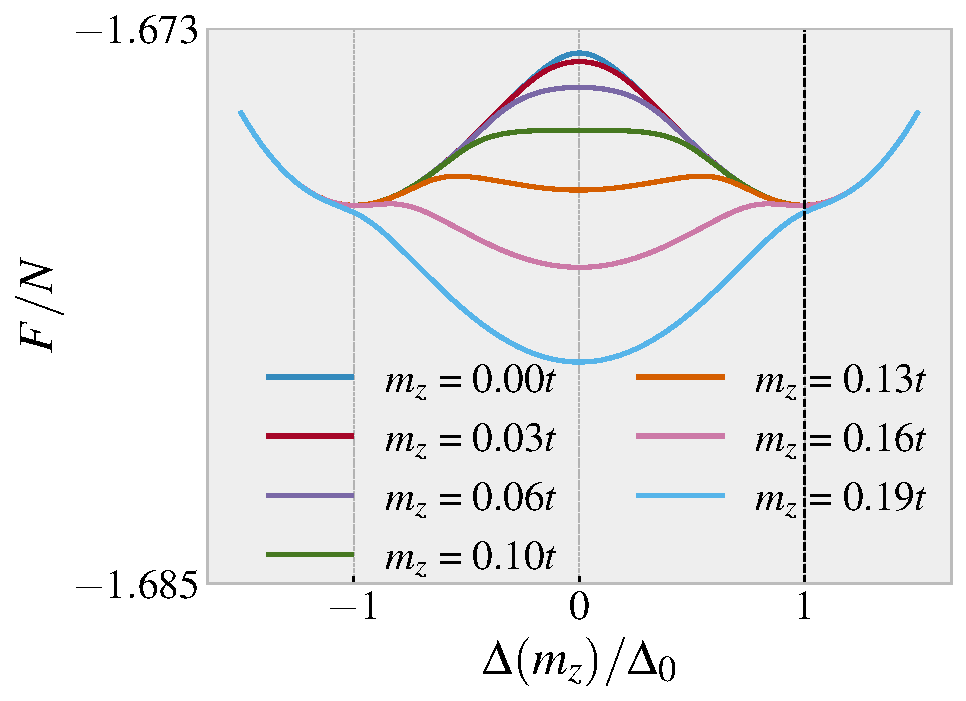
\includegraphics[width = \linewidth]{plots_maintext/F_h.pdf}
%     \end{subfigure}
%     \begin{subfigure}{0.9 \linewidth}
%         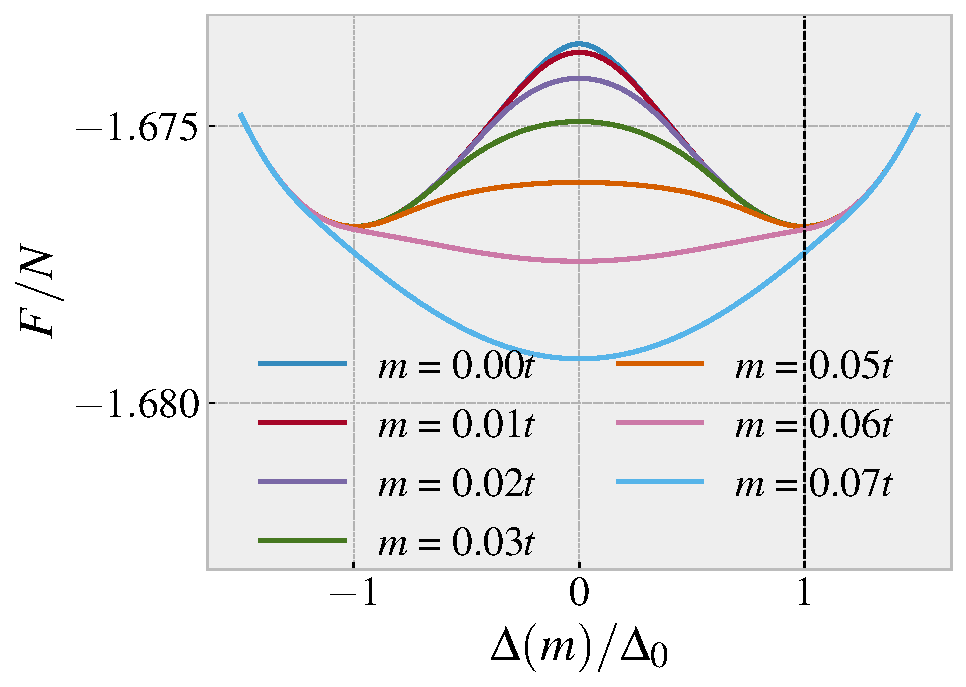
\includegraphics[width = \linewidth]{plots_maintext/F_m.pdf}
%     \end{subfigure}
%     \caption{Parameters used are $\mu = -0.5t$, $U = 1.7t$, $T = 0.02 \Delta_0$. The temperature is finite to avoid numerical errors. }
%     \label{fig:my_label}
% \end{figure}

% \begin{figure}[htb]
%     \centering
%     \begin{subfigure}{1.0 \linewidth}
%     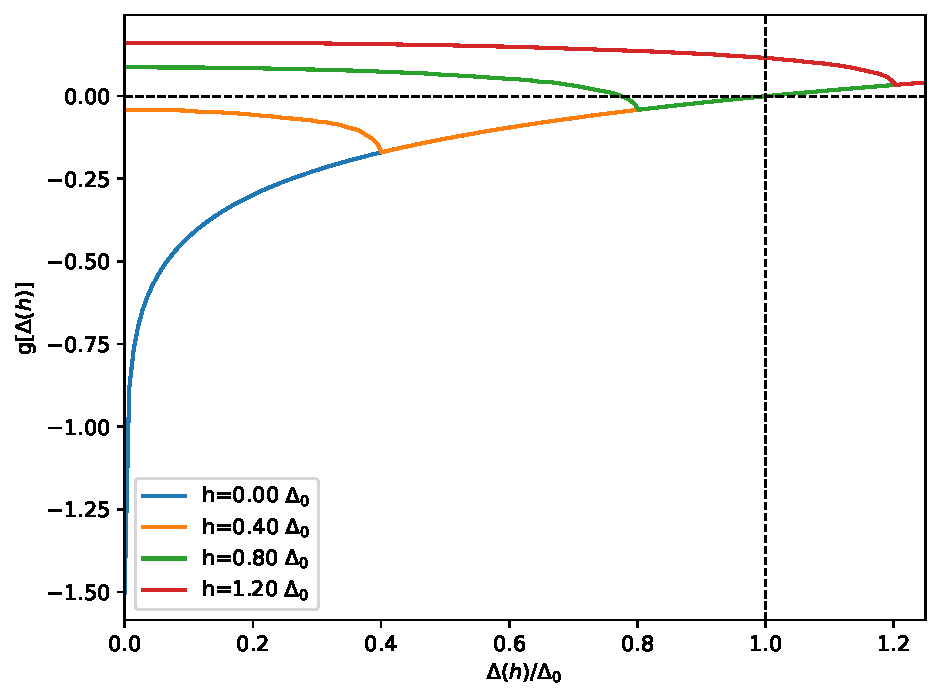
\includegraphics[width = \linewidth]{plots_maintext/g_h_mu=-2.pdf}
%     \end{subfigure}
%     \begin{subfigure}{1.0 \linewidth}
%     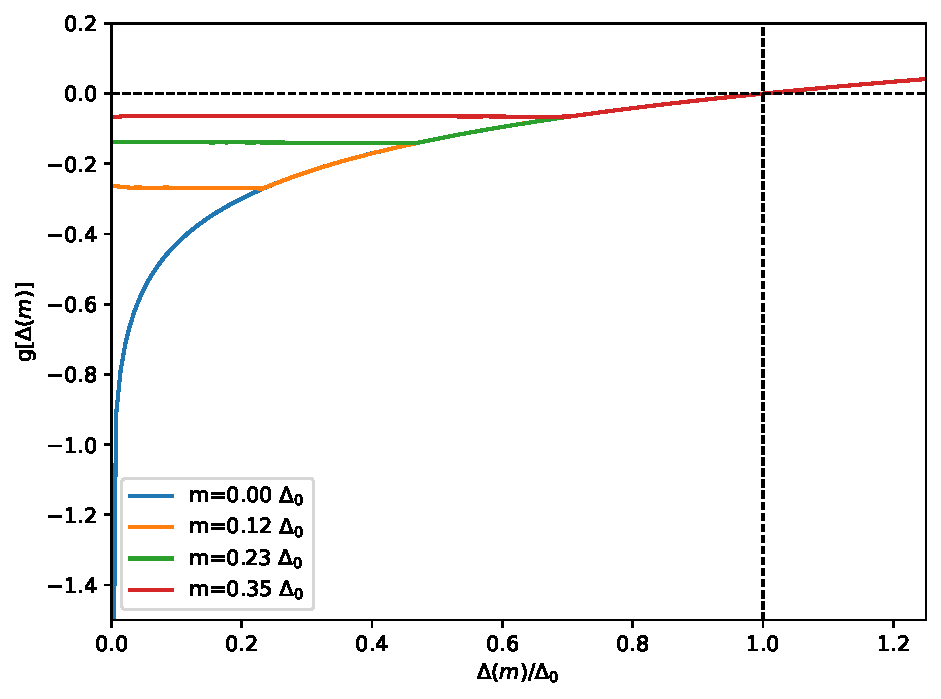
\includegraphics[width = \linewidth]{plots_maintext/g_m_mu=-2.pdf}
%     \end{subfigure}
%     \caption{The same as Fig. \ref{fig:g}, but for $\mu = -2 t$. In this case, we find $\Delta_0 =  0.04477$. This illustrates that in contrast to the FM case, the critical field in the AM depends on more than $\Delta_0$ (since in the $\mu = -0.5t$ case, there were no solutions for $m = 0.35 \Delta_0$, but here there is.}
%     \label{fig:g_mu=-2}
% \end{figure}
% \begin{figure}[htb]
%     \centering
%     \begin{subfigure}{1.0 \linewidth}
%     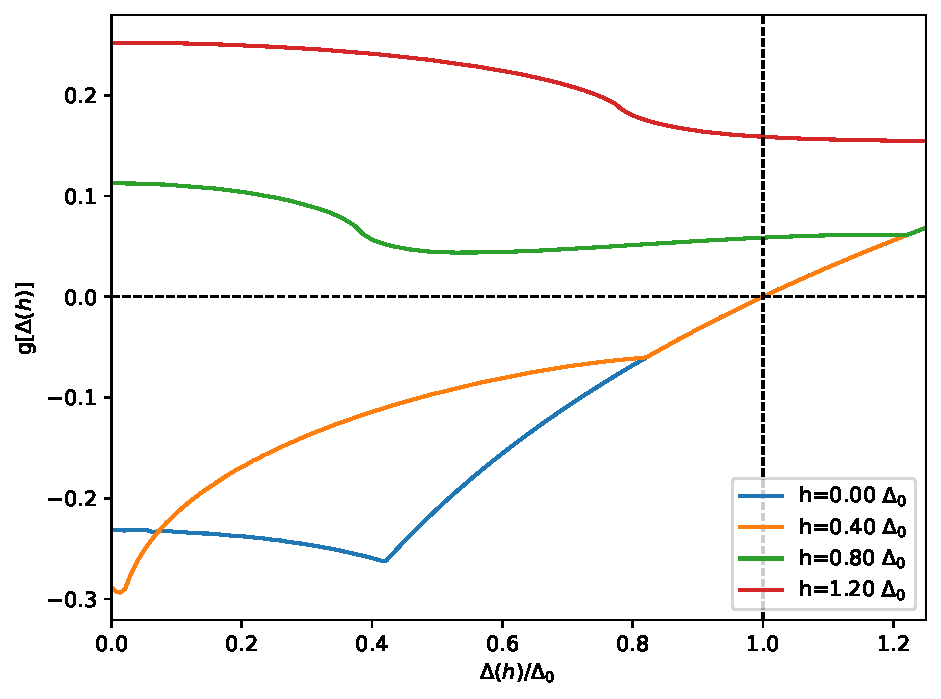
\includegraphics[width = \linewidth]{plots_maintext/g_h_mu=-0.5_m=0.02.pdf}
%     \end{subfigure}
%     \begin{subfigure}{1.0 \linewidth}
%     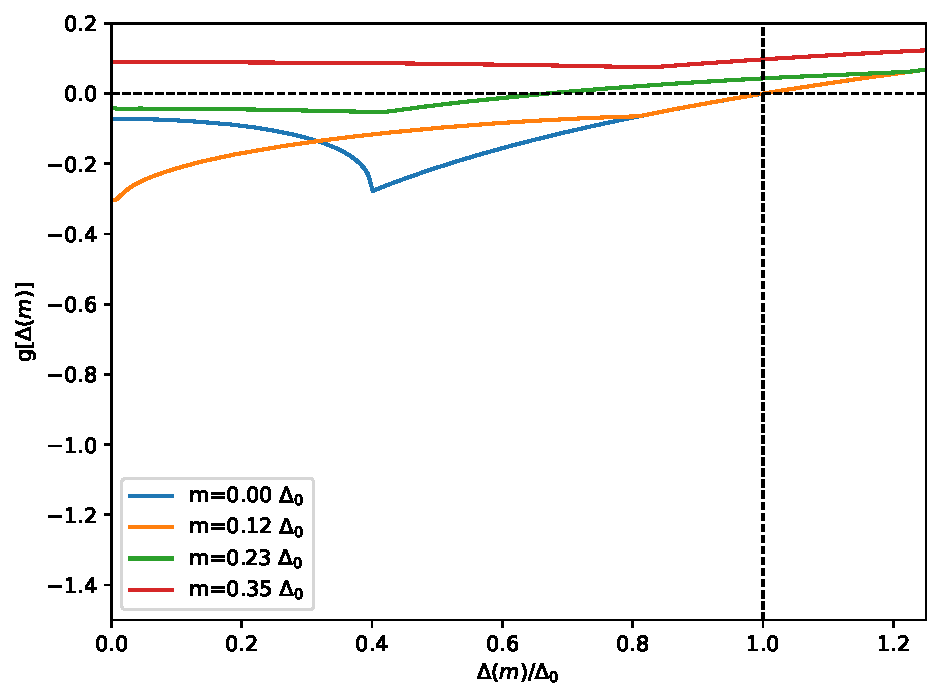
\includegraphics[width = \linewidth]{plots_maintext/g_m_mu=-0.5_h=0.08.pdf}
%     \end{subfigure}
%     \caption{Similar to Fig. \ref{fig:g}, but where both FM and AM fields are present. In the first plot, $m = 0.12 \Delta_0$,and in the second plot, $h = 0.4 \Delta_0$}
%     \label{fig:g_m+h}
% \end{figure}
\textit{Junction geometry}---
Using a square lattice, we consider two different AM/SC geometries: a straight junction, where the interface is aligned with the crystallographic axis, and a skewed junction, where the interface is rotated $45^\circ$ compared with the crystallographic axis. The two geometries are shown in Fig. \ref{fig:geometries}.
In the straight junction, hopping across the interface happens only along the $x$-axis, while in the skewed junction, hopping across the interface happens along both the $x$- and $y$- axis. 
\begin{figure}[htb]
    \begin{subfigure}[c]{0.15\linewidth}
    \vspace{5em}
        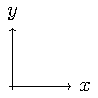
\includegraphics[width = \linewidth]{plots_maintext/coord.pdf}
    \end{subfigure}
    \hspace{1em}
    \begin{subfigure}[t]{0.35 \linewidth}
        \Large a)
    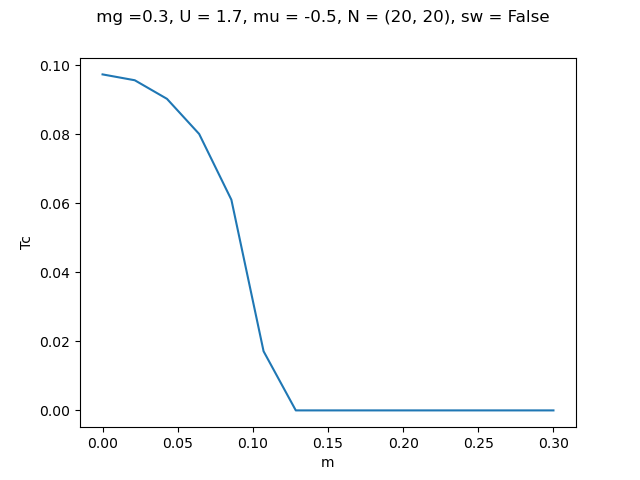
\includegraphics[width = \linewidth]{system_figures/straight.pdf}
    \end{subfigure}
    \hspace{2em}
    \begin{subfigure}[t]{0.3 \linewidth}
        \Large b)
    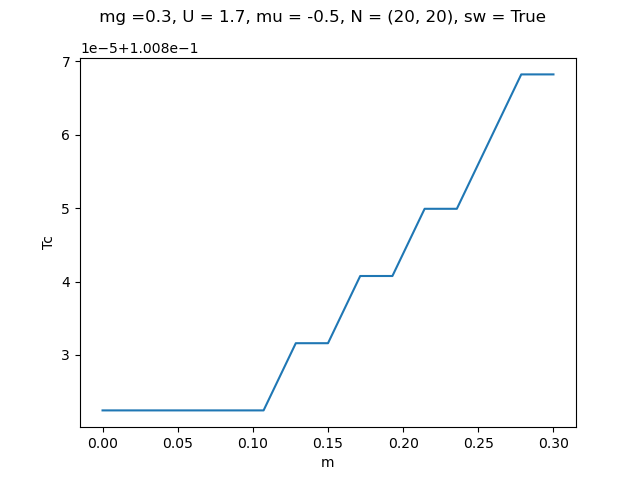
\includegraphics[width = \linewidth]{system_figures/skewed.pdf}
    \end{subfigure}
%     \begin{subfigure}{0.35 \linewidth}
% \Large d)
%         \includegraphics[width=\linewidth]{system_figures/spinup.pdf}
%     \end{subfigure}
%     \begin{subfigure}{0.35 \linewidth}
%     \Large e)
%         \includegraphics[width=\linewidth]{system_figures/spindown.pdf}
%     \end{subfigure}
    \caption{The two geometries of AM/SC junctions. In the straight junction in a), all interface hopping happens along the $x$-axis, while in the skewed junction in b), interface hopping happens (equal amount) along the $x$- and $y$-axis. }
    \label{fig:geometries}
\end{figure}
The (inverse) proximity effect in the SC-AM system can be understood by calculating the critical temperature $T_c$ in the SC. The result is shown in Fig. \ref{fig:geometry}. In the straight junction, superconductivity is suppressed \hans{comment more on supression/oscillation for final results} by the altermagnet, as Cooper pairs are split up by the leakage of electrons into the magnet. Since spin-up electrons favor hopping in the $x$-direction, they are trapped in the altermagnet for large $m$. In the skewed junction, this effect is averaged out, and the effects on $T_c$ are minimal. 
\begin{figure}[htb]
    \centering
    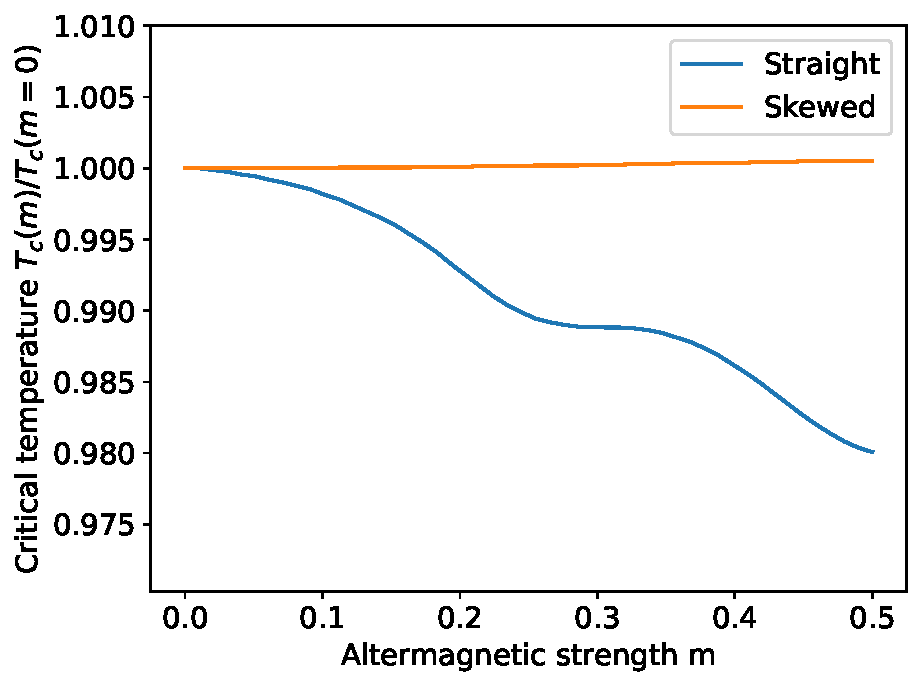
\includegraphics[width = 0.7 \linewidth]{plots_maintext/geometry.pdf}
    \caption{ The critical temperature for the two different junction geometries with $N_x = $, $N_y = $, and $N_\Delta = $.
    The critical temperatures are normalized to the zero-altermagnetism case for the two different junctions. Note that the critical temperatures are different in the two junctions: in the straight case it is $T_c(m = 0) = 0.098$, and in the skewed case $T_c(m = 0) = 0.12$. \hans{COMMENT: I expect the difference to go down when I run for a larger system in the end.}}
    \label{fig:geometry}
\end{figure}
% \begin{figure}
%     \centering
%     % \includegraphics{}
%     \caption{Caption}
%     \label{fig:my_label}
% \end{figure}

\textit{AM/SC/AM heterostructures.}---
An interesting extension to the discussion above can be achieved by adding another altermagnet to the AM/SC system considered above. We consider two situations: one where the two altermagnets are aligned and one where the second altermagnet is rotated by $90 ^ \circ$, and refer to these situations as a parallel (P) and antiparallel (AP) alignment.
Rotating the second altermagnet is analogous to changing the sign of $m$ in this region.
In Fig. \ref{fig:PAP}, the critical temperature of the SC is calculated for different values of $m$ in the two different systems.
In the P alignment, the situation is analogous to the AM/SC system considered above, and we see a similar pattern for suppression of $T_c$ for increasing altermagnetic strength $m$. \hans{COMMENT: Check the particle density, and see if there are fewer spin-up than spin-down electrons in the SC.  }
In the AP alignment case, one might naively expect the effects of the magnets to average out, resulting in less suppression of superconductivity. 
Surprisingly, as is evident from Fig.~\ref{fig:PAP}, $T_c$ is lower in the AP alignment than in the P alignment.
We attribute this to the appearance of \hans{(inverse)?} crossed Andreev reflection (CAR), sometimes referred to as nonlocal Andreev reflection.
It is well known that for a FSF heterostructure, the AP alignment of ferromagnets gives enhanced CAR compared to the AP alignment \cite{deutscher_apl_00}
\hans{COMMENT: add discussion of crossed Andreev reflections}
crossed Andreev reflections? 
\begin{figure}
    \centering
    \begin{subfigure}{0.6 \linewidth} 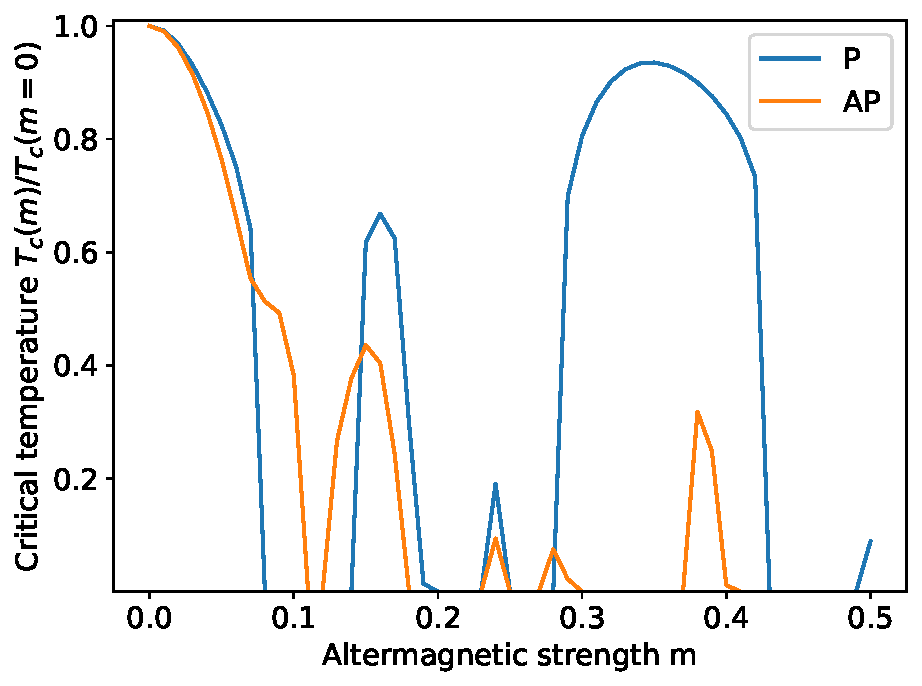
\includegraphics[width = \linewidth]{plots_maintext/PAPNx=30.pdf}
    \end{subfigure}
    \begin{subfigure}{0.6 \linewidth} 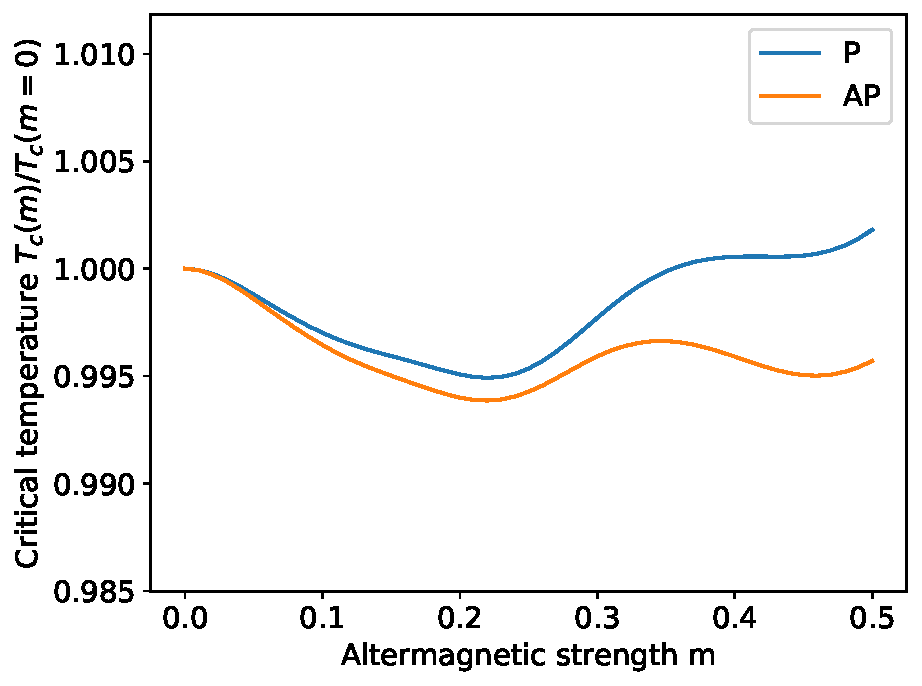
\includegraphics[width = \linewidth]{plots_maintext/PAPNx=40.pdf}
    \end{subfigure}
    \caption{The critical temperature in the AM/SC/AM system with P and AP alignment of the altermagnets. In the upper plot, the length of the SC is $10$, meaning that the SC is really short. In the lower plot, the length of the SC is $20$, so the effect is smaller. In both plots, the altermagnets on either side have a length of $10$. Other parameters are $N_y = 10$, $U = 1.7t$, $\mu = -0.5t$ \hans{To Do: run for $Nx = $}\hans{COMMENT: will run this with more values, and also for different lengths of the system. I think the length of the SC is critical here, so will do it for some systems where the altermagnet is stronger as well.}}
    \label{fig:PAP}
\end{figure}

\textit{Impurity scattering.}---
Materials with strong impurity scattering are highly relevant for experiments. 
For this reason, we include impurities $w_i = 1.0 t$ at randomly chosen positions in the altermagnet and study the effects on the critical temperature. 
We set the fraction of sites with impurities to $0.2$, and perform the calculations for $100$ different impurity configurations, before averaging over the resulting values of the critical temperature.
The fluctuations are defined as
\begin{equation}
    \delta T_c = \sqrt{\langle T_c^2 \rangle_{imp} - \langle T_c \rangle_{imp}^2},
\end{equation}
where the averages are taken over the $100$ impurity configurations.
In Fig. \ref{fig:imps}, the impurity calculations are shown for \hans{insert spesifications}. 
The results show that \hans{insert whether or not $T_c$ is affected more or less than in the $m=0 case$.}

\hans{Hypothesis: altermagnetism should be destroyed by strong impurity scattering. But this was based on arguments where we assumed a spherical Fermi surface...}
\hans{looks more like the results are minimal}
\begin{figure}[htb]
    \centering
    \begin{subfigure}{0.6 \linewidth}
        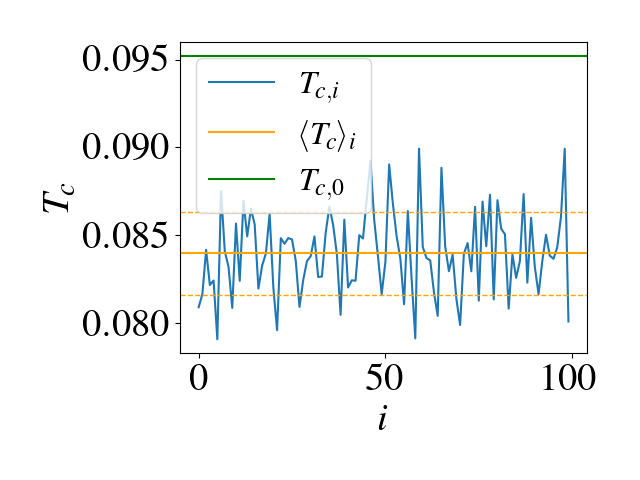
\includegraphics[width = \linewidth]{plots_maintext/imps1.png}
    \end{subfigure}
    \caption{The critical temperature in a $N_x^{AM} = N_x^{SC}=10$, $N_y=20$ when including impurities with $w^{AM} = 1.0t$ and $N_{i}^{AM} =0.2$. The calculated value without impurities is shown in green, and the average impurity value and standard deviation are shown in orange. To the left, the normal-metal case $m=0$. Here, $\langle T_c \rangle_{i} = 0.084$, and $\delta T_c = 0.0024$. To the right, $m = 0.5t$. }
    \label{fig:imps}
\end{figure}
\begin{comment}
    \begin{figure}
    \centering
    \begin{subfigure}{0.6 \linewidth}
        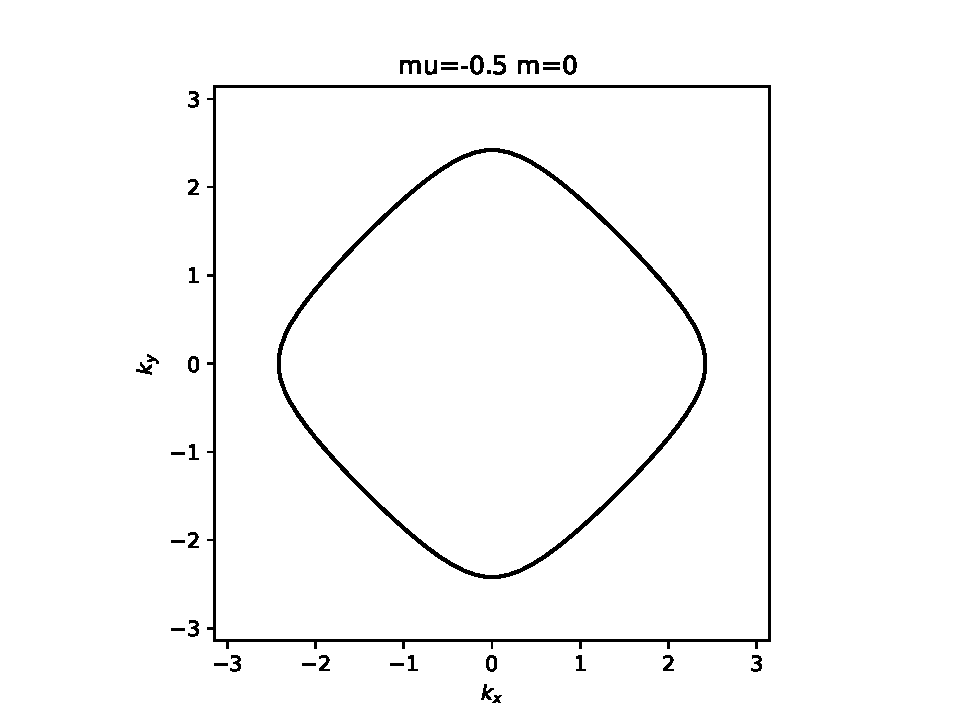
\includegraphics[width = \linewidth]{plots_maintext/FS1.pdf}
    \end{subfigure}
    \begin{subfigure}{0.6 \linewidth}
        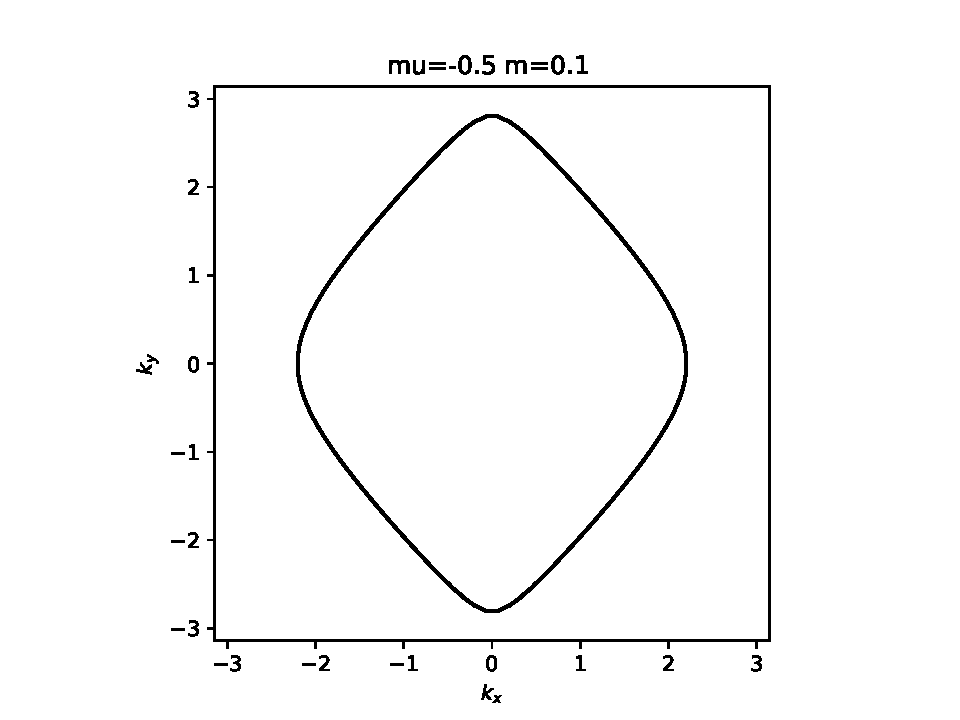
\includegraphics[width = \linewidth]{plots_maintext/FS2.pdf}
    \end{subfigure}
    \begin{subfigure}{0.6 \linewidth}
        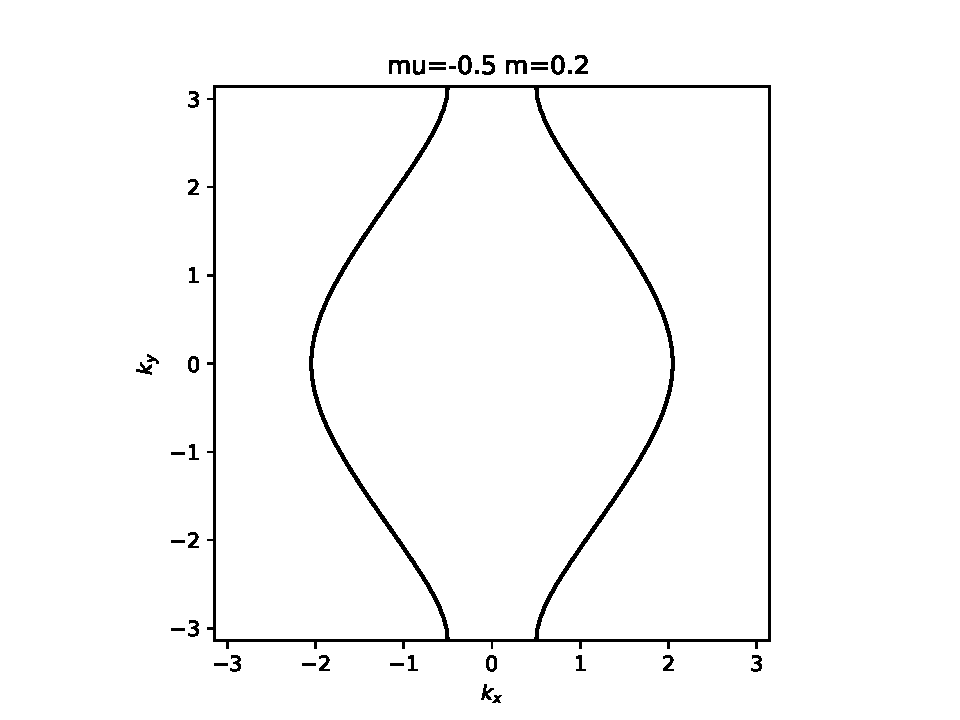
\includegraphics[width = \linewidth]{plots_maintext/FS3.pdf}
    \end{subfigure}
    \caption{The Fermi surface ( without SC) $\xi_k - 2m (\cos k_x - \cos k_y) = \mu$ for different $m$. The chemical potential is $\mu = -0.5 t$, the same as in the simulations.}
    \label{fig:FS}
\end{figure}
\end{comment}
\acknowledgments

 

This work was supported by the Research
Council of Norway through Grant No. 323766 and its Centres
of Excellence funding scheme Grant No. 262633 “QuSpin.”


\begin{thebibliography}{999}

\bibitem{hirohata_jmmm_20}
	A.~Hirohata, K.~Yamada, Y.~Nakatani, I.-L.~Prejbeanu, B.~Dieny, P.~Pirro, B.~Hillebrands.
	J.~Mag.~Mag.~Mater.~\textbf{509}, 166711 (2020).



\bibitem{ahn_prb_19} K.-H. Ahn, A. Hariki, K.-W. Lee, and J. Kunes,  Phys. Rev. B \textbf{99}, 184432 (2019)

\bibitem{hayami_jpsj_19} S. Hayami, Y. Yanagi, and H. Kusunose, J. Phys. Soc. Jpn. \textbf{88}, 123702 (2019).


\bibitem{yuan_prb_20}
	L.-D.~Yuan, Z.~Wang, J.-W.~Luo, E.~I.~Rashba, and A.~Zunger.
	Phys.~Rev.~B \textbf{102}, 014422 (2020).

\bibitem{smejkal_sciadv_20}
	L.~Šmejkal, R.~González-Hernández, T.~Jungwirth, and J.~Sinova.
	Sci.~Adv.~\textbf{6}, 8809 (2020).


\bibitem{smejkal_prx_perspective_22} L. Šmejkal, J. Sinova, and T. Jungwirth, Phys. Rev. X \textbf{12}, 040501 (2022).

	\bibitem{reichlova_arxiv_20}
	H.~Reichlova, R.L.~Seeger, R.~González-Hernández, I.~Kounta, R.~Schlitz, D.~Kriegner, P.~Ritzinger, M.~Lammel, M.~Leiviskä, V.~Petiček, P.~Doležal, E.~Schmoranzerova, A.~Badura, A.~Thomas, V.~Baltz, L.~Michez, J.~Sinova, S.~T.~B.~ Goennenwein, T.~Jungwirth, and L.~Smejkal.
	arXiv:2012.15651.

	\bibitem{smejkal_prx_22}
	L.~Šmejkal, J.~Sinova, and T.~Jungwirth, Phys.~Rev.~X \textbf{12}, 031042 (2022).

	\bibitem{lopez-moreno_pccp_16}
	S.~Lopez-Moreno, A.~H.~Romero, J.~Mejia-Lopez, and A.~Muñoz.
	Phys.~Chem.~Chem.~Phys.~\textbf{18}, 33250 (2016).

	\bibitem{pekar_zetf_64}
	S.~I.~Pekar and E.~I.~Rashba.
	Zh.~Eksp.~Teor.~Fiz.~\textbf{47}, 1927 (1964).

	\bibitem{clarke_prsa_69}
	J.~Clarke.
	Proc.~Roy.~Soc.~A \textbf{308}, 447 (1969).

	\bibitem{oda_ssc_80}
	Y.~Oda and H.~Nagano.
	Sol.~State Com.~\textbf{35}, 631 (1980).

	\bibitem{ryazanov_prl_01}
	V.~V.~Ryazanov, V.~A.~Oboznov, A.~Yu.~Rusanov, A.~V.~Veretennikov, A.~A.~Golubov, and J.~Aarts.
	Phys.~Rev.~Lett.~\textbf{86}, 2427 (2001).

	\bibitem{buzdin_rmp_05}
	A.~I.~Buzdin.
	Rev.~Mod.~Phys.~\textbf{77}, 935 (2005).

	\bibitem{ioffe_nature_99}
	L.~Ioffe, V.~Geskenbein, M.~Feigelman, A.~Fauchere, and G.~Blatter.
	Nature \textbf{398}, 679–681 (1999).

	\bibitem{feofanov_natphys_10}
	A.~K.~Feofanov, V.~A.~Oboznov, V.~V.~Bol’ginov, J.~Lisenfeld, S.~Poletto, V.~V.~Ryazanov, A.~N.~Rossolenko, M.~Khabipov, D.~Balashov, A.~B.~Zorin, P.~N.~Dmitriev, V.~P.~Koshelets, and A.~V.~Ustinov.
	Nat.~Phys.~\textbf{6}, 593 (2010).

	\bibitem{geshkenbein_pisma_86}
	V.~Geshkenbein and A.~Larkin.
	Pis'ma Zh.~Eksp.~Teor.~Fiz.~\textbf{43}, 306 (1986).

	\bibitem{millis_prb_88}
	A.~Millis, D.~Rainer, and J.~A.~Sauls.
	Phys.~Rev.~B \textbf{38}, 4504 (1988).

	\bibitem{szombati_natphys_16}
	D.~B.~Szombati, S.~Nadj-Perge, D.~Car, S.~R.~Plissard, E.~P.~A.~M.~Bakkers, L.~P.~Kouwenhoven.~
	Nat.~Phys.~\textbf{12}, 568 (2016).

	\bibitem{andersen_prl_06}
	B.~Andersen, I.~Bobkova, P.~Hirschfeld, and Yu.~Barash.
	Phys.~Rev.~Lett.~\textbf{96}, 117005 (2006).

	\bibitem{zhu2016}
	J.-X. Zhu.
	Bogoliubov–de Gennes method and its applications (2016).

	\bibitem{degennes1966}
	P.~G. de~Gennes.
	Superconductivity of metals and alloys (1966).

	\bibitem{weisse2006}
	A.~Weiße, G.~Wellein, A.~Alvermann, H.~Fehske.
	Rev.~Mod.~Phys. \textbf{78}, 275 (2006).

 \bibitem{bhowal_arxiv_22} S. Bhowal and N. A. Spaldin, arXiv:2212.03756
 

	\bibitem{covaci2010}
	L.~Covaci, F.~M.~Peeters and M.~Berciu.
	Phys.~Rev.~Lett. \textbf{105}, 167006 (2010).

	\bibitem{nagai2012}
	Y.~Nagai, Y.~Ota and M.~Machida.
	J.~Phys.~Soc.~Jpn. \textbf{81}, 024710 (2012).

	\bibitem{goedecker1999}
	S.~Goedecker.
	Rev.~Mod.~Phys. \textbf{71}, 1085 (1999).

	\bibitem{benfenati2022}
	A.~L.~Benfenati.
	Numerical solutions to non-linear inhomogeneous problems in superconductivity.
	PhD thesis (KTH, 2022).

\bibitem{li_prl_13} Bin Li, Niklas Roschewsky, Badih A. Assaf, Marius Eich, Marguerite Epstein-Martin, Don Heiman, Markus Münzenberg, and Jagadeesh S. Moodera
Phys. Rev. Lett. \textbf{110}, 097001 (2013)

\bibitem{singh_prx_15} A. Singh \etal, Phys. Rev. X \textbf{5}, 021019 (2015)

\bibitem{clogston_prl_62} A. M. Clogston,  . Upper Limit for the Critical Field in Hard Superconductors. Physical Review Letters, 9(6), 266–267 (1962).

\bibitem{ouassou_19} Ouassou, J. A. . Manipulating superconductivity in magnetic nanostructures in and out of equilibrium. PhD thesis (NTNU, 2019).

\bibitem{chandrasekhar_apl_62} B. S. Chandrasekhar. A note on the maximum critical field of high-field superconductors. Applied Physics Letters, 1(1), 7–8 (1962).

\bibitem{deutscher_apl_00} Guy Deutscher, Denis Feinberg; Coupling superconducting-ferromagnetic point contacts by Andreev reflections. Applied Physics Letters 76 (4): 487–489. (2000).
% https://doi.org/10.1063/1.125796

\bibitem{ouassou_arx_23} J. A. Ouassou, A. Brataas, and J. Linder. (2023). Josephson effect in altermagnets (arXiv:2301.03603). arXiv. \url{http://arxiv.org/abs/2301.03603}.


\bibitem{sun_arx_23} C. Sun, A. Brataas, J. Linder (2023) Andreev reflection in altermagnets ( arXiv:2303.14236v2) arXiv. \url{https://arxiv.org/abs/2303.14236}
\end{thebibliography}




\end{document}
